\newif\ifdraft
\newif\iffull
\newif\ifcomment
\newif\iflatexdiff
\newif\ifbibtex
\newif\ifpreprint
%
\latexdifftrue %enable latex diff commands
\drafttrue     %enable draft banner and version number
\bibtextrue    %enable bibtex (off for final preprint or paper)
\preprinttrue  %enable cern preprint (for arXiv)
%fulltrue      %include author and acknowledgement and references (refpaper.tex/refpreprint.tex)
%
\newif\ifplbpaper
\newif\ifapspaper
\apspapertrue
%
\def\snntitle{$\snn$}
\ifpreprint
  \def\snntitle{$\snnbf$}
\fi
%
\def\dtitle{$\Lambda$ and $\Kshort$ in jets in p--Pb collisions at $\sNN=5.02$~TeV}
\def\stitle{$\Lambda$ and $\Kshort$ in jets} % Put a short paper title (only relevant for CERN paper)
\def\phnum{2015-XXX}     % Required, obtained from PH
\def\phdat{xx yyy 2015}  % Required, obtained from PH
\def\dvers{v2.0}         % Set version number by hand every time you want to change it
\def\revision{rev. 1}
%
\ifpreprint
  \documentclass[ALICE,manyauthors,12pt]{cernphprep}
  \usepackage[comma,square,numbers,sort&compress]{natbib}
  \usepackage{booktabs}
\else %%% PUT PAPER STYLE BELOW %%%
  \ifplbpaper
  \documentclass[final,3p,12pt]{elsarticle}
  \biboptions{comma,square,numbers,sort&compress}
  \def\bibstname{utphys}
  \fi
%
  \ifapspaper
  \documentclass[10pt,aps,prl,superscriptaddress,altaffilletter,nobibnotes,nofootinbib]{revtex4-1}
  \newenvironment{frontmatter}{}{\maketitle}
  \def\bibstname{apsrev4-1}
  \fi
\fi
%%%%%%%%%%%%%%%%%%%%%%%%%%%%%%%%%%%%%%%%%%%%%%%%%%%%%%%%%%%%%%%%%%%%%%%%%%%%%%%

\ifdraft
  \usepackage{lineno}
  \linenumbers
  \setlength\linenumbersep{0.06in}
  \modulolinenumbers[5]
  \usepackage{fancyhdr}
  \pagestyle{fancyplain}
  \fancyhead{}
  \fancyhead[L,L]{\color{red}ALICE INTERNAL ONLY}
  \fancyhead[R,R]{\thepage}
  \fancyfoot{}
  \fancyfoot[L,L]{\color{red}DRAFT \dvers\ \revision $\color{white}:$\$}
  \fancyfoot[R,R]{\color{red} \today $\color{white}:$\$}
  \renewcommand{\headrulewidth}{0pt} % remove lines as well
  \renewcommand{\footrulewidth}{0pt}
  \newcommand{\ask}[1]{\textcolor{magenta}{#1}}
\else
  \newcommand{\ask}[1]{}
\fi
%%%%%%%%%%%%%%%%%%%%%%%%%%%%%%%%%%%%%%%%%%%%%%%%%%%%%%%%%%%%%%%%%%%%%%%%%%%%%%%

\iflatexdiff
  \RequirePackage{color}
  \definecolor{RED}{rgb}{1,0,0}
  \definecolor{BLUE}{rgb}{0,0,1}
  \providecommand{\DIFadd}[1]{{\protect\color{blue}\uwave{#1}}}
  \providecommand{\DIFdel}[1]{{\protect\color{red}\sout{#1}}}
  \providecommand{\DIFaddbegin}{}
  \providecommand{\DIFaddend}{}
  \providecommand{\DIFdelbegin}{}
  \providecommand{\DIFdelend}{}
  \providecommand{\DIFaddFL}[1]{\DIFadd{#1}}
  \providecommand{\DIFdelFL}[1]{\DIFdel{#1}}
  \providecommand{\DIFaddbeginFL}{}
  \providecommand{\DIFaddendFL}{}
  \providecommand{\DIFdelbeginFL}{}
  \providecommand{\DIFdelendFL}{}
\fi
%==========================================================%

\usepackage{float}
\usepackage{rotating}

\usepackage{graphicx}
\usepackage{graphics}
\usepackage{epstopdf}
\usepackage{epsfig}
\usepackage{grffile}

\usepackage{dcolumn}
\usepackage{multirow}
\usepackage{array}

\usepackage{bm}
\usepackage{amsmath}
\usepackage{amssymb}
\usepackage{amsfonts}

\usepackage{units}
\usepackage{hyperref}

\usepackage{color}
%\usepackage[usenames]{color}

\usepackage{textcomp}
\usepackage[normalem]{ulem}
\usepackage[utf8]{inputenc}
\usepackage[T1]{fontenc}

%usepackage{changes}
%usepackage{lipsum}
%definechangesauthor[name={Xiaoming Zhang}, color=orange]{xz}
%definechangesauthor[name={MP}, color=orange]{mp}
%setremarkmarkup{(#2)}
%%%%%%%%%%%%%%%%%%%%%%%%%%%%%%%%%%%%%%%%%%%%%%%%%%%%%%%%%%%%%%%%%%%%%%%%%%%%%%%

\graphicspath{{figures/}
              {figures/c00Logos/}
              {figures/c23V0Reco/}
              {figures/c24Syst/}
              {figures/c03Results/}}
%%%%%%%%%%%%%%%%%%%%%%%%%%%%%%%%%%%%%%%%%%%%%%%%%%%%%%%%%%%%%%%%%%%%%%%%%%%%%%%

\newcolumntype{P}[1]{>{\centering\arraybackslash}p{#1}}
\newcolumntype{M}[1]{>{\centering\arraybackslash}m{#1}}
%%%%%%%%%%%%%%%%%%%%%%%%%%%%%%%%%%%%%%%%%%%%%%%%%%%%%%%%%%%%%%%%%%%%%%%%%%%%%%%

\newcommand{\murm}{%
  \ifmmode
    \mathchoice
        {\hbox{\normalsize\textmu}}
        {\hbox{\normalsize\textmu}}
        {\hbox{\scriptsize\textmu}}
        {\hbox{\tiny\textmu}}%
  \else
    \textmu
  \fi
}
%%%%%%%%%%%%%%%%%%%%%%%%%%%%%%%%%%%%%%%%%%%%%%%%%%%%%%%%%%%%%%%%%%%%%%%%%%%%%%%

\newcommand{\pip}{\ensuremath{\pi^{+}}}
\newcommand{\pim}{\ensuremath{\pi^{-}}}
\newcommand{\kap}{\ensuremath{{\rm K}^{+}}}
\newcommand{\kam}{\ensuremath{{\rm K}^{-}}}
\newcommand{\pbar}{\ensuremath{\rm\overline{p}}}
\newcommand{\degree}{\ensuremath{^{\rm o}}}
\newcommand{\s}{\ensuremath{\sqrt{s}}}
\newcommand{\pt}{\ensuremath{p_{\rm t}}}
\newcommand{\dedx}{\ensuremath{{\rm d}E/{\rm d}x}}
\newcommand{\dndy}{\ensuremath{{\rm d}N/{\rm d}y}}
\newcommand{\dndydpt}{\ensuremath{{\rm d}^{2}N/{\rm d}y{\rm d}p_{\rm t}}}
\newcommand{\pp}{pp}

\newcommand{\jpsi}{\ensuremath{{\rm J/}\psi}}
\newcommand{\psip}{\ensuremath{\psi^{\prime}}}
\newcommand{\jpsiDY}{\ensuremath{{\rm J/}\psi{\rm ,/,DY}}}
\newcommand{\dd}{\ensuremath{{\rm d}}}
\newcommand{\chic}{\ensuremath{\chi_{\rm c}}}
\newcommand{\ezdc}{\ensuremath {E_{\rm ZDC}}}
\newcommand{\red}{\textcolor{red}}
\newcommand{\blue}{\textcolor{blue}}

\newcommand{\slfrac}[2]{\left.#1\right/#2}
%%%%%%%%%%%%%%%%%%%%%%%%%%%%%%%%%%%%%%%%%%%%%%%%%%%%%%%%%%%%%%%%%%%%%%%%%%%%%%%

\newcommand{\abs}[1]{\ensuremath{\left|#1\right|}}
\newcommand{\avg}[1]{\ensuremath{\left\langle #1\right\rangle}}

\newcommand{\pT}[1][T]{\ifthenelse{\equal{#1}{T}}
                                  {\ensuremath{p_{\rm #1}}}
                                  {\ensuremath{p_{\rm T,#1}}}}

\newcommand{\dndydpT}{\ensuremath{{\rm d}^{2}N/{\rm d}y{\rm d}p_{\rm T}}}
\newcommand{\dtod}[2]{\ensuremath{{\rm d}#1/{\rm d}#2}}
\newcommand{\dtodd}[3]{\ensuremath{{\rm d}^{2}#1/{\rm d}#2{\rm d}#3}}
%%%%%%%%%%%%%%%%%%%%%%%%%%%%%%%%%%%%%%%%%%%%%%%%%%%%%%%%%%%%%%%%%%%%%%%%%%%%%%%

\newcommand{\GeVc} {\ensuremath{{\rm GeV/}c}}
\newcommand{\GeVcc}{\ensuremath{{\rm GeV/}c^{2}}}

\newcommand{\MeVc} {\ensuremath{{\rm MeV/}c}}
\newcommand{\MeVcc}{\ensuremath{{\rm MeV/}c^{2}}}

\newcommand{\sNN}{\ensuremath{\sqrt{s_{\rm NN}}}}
\newcommand{\hlab}{\ensuremath{\eta_{\rm lab}}}
\newcommand{\yCMS}{\ensuremath{y_{\rm CMS}}}
\newcommand{\yNN}{\ensuremath{y_{\rm NN}}}

\newcommand{\kT}{\ensuremath{k_{\rm T}}}
\newcommand{\Ajet}{\ensuremath{A_{\rm jet}}}
\newcommand{\RAA}{\ensuremath{R_{\rm AA}}}

\newcommand{\Vzero}{\ensuremath{{\rm V}^{0}}}
\newcommand{\Kshort}{\ensuremath{{\rm K}_{\rm S}^{0}}}
\newcommand{\AntiLa}{\ensuremath{\overline{\Lambda}}}

\newcommand{\qhat}{\ensuremath{\hat{q}}}
\newcommand{\cent}[2]{$#1$--$#2\%$}
%%%%%%%%%%%%%%%%%%%%%%%%%%%%%%%%%%%%%%%%%%%%%%%%%%%%%%%%%%%%%%%%%%%%%%%%%%%%%%%

%%%%%%%%%%%%%%%%%%%%%%%%%%%%%%%%%%%%%%%%%%%%%%%%%%%%%%%%%%%%%%%%%%%%%%%%%%%%%%%

\begin{document}

\ifpreprint
  \begin{titlepage}
  \PHnumber{\phnum}
  \PHdate{\phdat}
  \title{\dtitle}
  \ShortTitle{\stitle}
%
  \iffull
    \Collaboration{ALICE Collaboration~\thanks{See Appendix~\ref{app:collab} for the list of collaboration members}}
  \else
    \Collaboration{ALICE Collaboration}
  \fi
%
  \ShortAuthor{ALICE Collaboration}
%
  \ifdraft
    \begin{center}
    \today\\ \color{red}DRAFT \dvers\ \hspace{0.3cm} \revision $\color{white}:$\$\color{black}\vspace{0.3cm}
    \end{center}
  \fi
\else
  \begin{frontmatter}
  \title{\dtitle}
%
  \iffull
    \input{authors-paper.tex}
    \Collaboration{ALICE Collaboration}
  \else
    \ifdraft
      \author{ALICE Collaboration \\ \vspace{0.3cm}
      \today\\ \color{red}DRAFT \dvers\ \hspace{0.3cm} \revision $\color{white}:$\$\color{black}}
    \else
      \author{ALICE Collaboration}
    \fi
  \fi
\fi
%%%%%%%%%%%%%%%%%%%%%%%%%%%%%%%%%%%%%%%%%%%%%%%%%%%%%%%%%%%%%%%%%%%%%%%%%%%%%%%

\begin{abstract}
%!TEX root = ../AliPubV0JetspPb.tex
The production of \lda\ baryons and \ks\ mesons has been measured separately in hard scattering region and the underlying event in \pPb\ collisions at \sqrtsnn{5.02} at the LHC.
The hard scatterings are selected on an event-by-event basis by jets reconstructed using charged particles with \akT\ jet finder and resolution parameter $R=0.4$ (or $R=0.2$), and \ptjet\ of $10$ (or $20$)~\gevc.

The ratio of inclusive differential yields of \lda\ and \ks\ at intermediate transverse momentum (\pt) is much larger in the systems such as \PbPb\ and \pPb\ collisions as compared to \pp\ collisions. The increased ratio in \PbPb\ has been attributed to collective effects in those collisions. Recent studies have revealed qualitatively similar effects in high-multiplicity \pPb\ collisions.

In this letter, we report that in \pPb\ collisions the ratio of \lda\ to \ks\ associated to jets is consistent with \pp\ expectation given by PYTHIA event generator. Whereas, the ratio in the underlying event shows a prominent maximum (similar to the inclusive distribution) at the intermediate \pt\ of 2-5 \gevc. Moreover the yields in jets do not change with the event multiplicity, while the large baryon/meson ratio evolves and it is larger in events with the highest multiplicity as compared to minimum bias collisions.



\end{abstract}

\ifpreprint
  \end{titlepage}
\else
  \begin{keyword}
%% keywords here, in the form: keyword \sep keyword
%% MSC codes here, in the form: \MSC code \sep code
%% or \MSC[2008] code \sep code (2000 is the default)
  heavy-ion \sep collision \sep  LHC \sep  electron \sep heavy-flavour \sep suppression
  \end{keyword}
  \end{frontmatter}
  \newpage
\fi
%
\ifdraft
  \thispagestyle{fancyplain}
\fi
%
%%%%%%%%%%%%%%%%%%%%%%%%%%%%%%%%%%%%%%%%%%%%%%%%%%%%%%%%%%%%%%%%%%%%%%%%%%%%%%%

\section*{Log section:}

\thispagestyle{empty}

\ask{\bf Last agreement between PCs}
\begin{itemize}
\item \ask{Show the average results over various $R$ in MB events.}
\item \ask{Select some results in event activities and put in appendix.}
\item \ask{Some of the current figs will be updated with this definition.}
\end{itemize}

\ask{\bf Additional considerations}
\begin{itemize}
\item \ask{As a cross check, the $\Lambda$ and $\AntiLa$ were reconstructed separately in the analysis.}
\item \ask{Do we need to combine them in the paper?}
\item \ask{All the corresponding figures will be updated if it does.}
\end{itemize}

\ask{\bf Todo}
\begin{itemize}
\item \ask{Section~\ref{sec:Intro}: go back at the end with PCs.}
\item \ask{Section~\ref{sec:Results}: add the discussion of the results -- plots need to be updated.}
\item \ask{Section~\ref{sec:con}: to be finalized.}
\end{itemize}


\ask{\bf Modifications}
\begin{itemize}
\item \ask{Section~\ref{sec:EveSel} -- simplified the contents, do we need to put more info?}
\item \ask{Section~\ref{sec:JetReco} -- optimized the contents, text will be improved.}
\item \ask{Section~\ref{sec:V0Reco} -- simplified the text, improvements are needed.}
\item \ask{Section~\ref{sec:Syst} -- considering to add additional table(s) figure(s).}
\end{itemize}



\newpage

%%%%%%%%%%%%%%%%%%%%%%%%%%%%%%%%%%%%%%%%%%%%%%%%%%%%%%%%%%%%%%%%%%%%%%%%%%%%%%%

\setcounter{page}{2}

%!TEX root = ../AliPubV0JetspPb.tex

\section{Introduction}
%%\ask{Intro taken from the ID spectra mult dependence in p-Pb. Needs adjustments for the purpose of this paper.}

High-energy heavy ion collisions provide a unique opportunity to study
properties of hot and dense QCD medium composed of deconfined partons -
the quark-gluon plasma (QGP). The QGP is predicted by the lattice QCD
calculations \cite{Satz:2000bn,Bass:1998vz,Shuryak:1984nq,Cleymans:1985wb}. The cross-over transition from
hadronic matter to the QGP matter at zero
baryochemical potential is expected to take place once the
temperature of the matter $T_{c}$ reaches values of about 150 MeV and/or
energy density $\epsilon_{c}$ of about 0.5 GeV/fm$^3$ \cite{Borsanyi:2010cj,Bhattacharya:2014ara}. 
The measurements indicate that the most violent collisions of lead ions at the LHC at
\sqrtsnn{2.76}\ create conditions well above the critical temperature at approximately zero baryochemical potential.
The bulk matter created in those collisions can be
quantitatively described in terms of hydrodynamic and statistical
models. The initial hot and dense partonic matter rapidly expands and
cools down, ultimately undergoing a transition to a hadron gas
phase~\cite{Muller:2006ee}. During the expansion phase, collective hydrodynamic flow develops from
the initially generated pressure gradients in the strongly interacting
system. This results in a characteristic dependence of the shape of
the transverse momentum (\pt) distribution on the particle mass that
can be described using a common kinetic freeze-out temperature parameter \Tfo\
and a collective average expansion velocity
\avbT~\cite{Schnedermann:1993ws}.

The interpretation of heavy-ion results depends on the understanding of results from smaller collision
systems such as proton-proton (\pp) or proton-nucleus (pA). Proton-nucleus collisions are intermediate between
proton-proton and nucleus-nucleus collisions in terms of
system size and number of produced particles. Comparing particle
production in pp, pA, and AA reactions has frequently been used to
separate initial state effects, linked to the use of nuclear
beams or targets, from final state effects, associated to the presence of hot and
dense matter. At the LHC, however, the pseudorapidity density of final state
particles in pA collisions reaches values which can become
comparable to semi-peripheral Au--Au ($\sim$60\% most central) and Cu--Cu ($\sim$30\% most central) collisions at top RHIC energy~\cite{Alver:2010ck}.
Indeed, the measurements at the LHC in high-multiplicity pp and \pPb\ collisions have revealed unexpectedly strong long-range correlations of produced particles \cite{Khachatryan:2010gv,CMS:2012qk,Abelev:2012ola,Aad:2012gla,Aad:2013fja,Chatrchyan:2013nka} falsyfying the assumption that final state dense matter effects can be neglected in pA.

Various mechanisms have been proposed to explain the origin of this collective particle production. 
Both a Color Glass Condensate (CGC)
description~\cite{Dusling:2013oia}, based on initial state nonlinear
gluon interactions, as well as a model based on hydrodynamic
flow~\cite{Bozek:2012gr,Qin:2013bha}, assuming strong interactions
between final state partons or hadrons, can give a satisfactory
description of the \pPb\ correlation data. However, the modeling of
small systems such as \pPb\ is complicated because uncertainties
related to initial state geometrical fluctuations play a large role
and because viscous corrections may be too large for hydrodynamics to
be a reliable framework~\cite{Bzdak:2013zma}.

Results on identified particle production in \pPb\ collisions at a nucleon-nucleon center-of-mass energy \sqrtsnn{5.02} at the LHC \cite{Abelev:2013haa} have shown qualitatively similar effects as in AA collisions \cite{Abelev:2013xaa,ABELEV:2013wsa}. In particular the ratio of baryon and meson transverse momentum (\pt) spectra shows a pronounced maximum at intermediate \pt. The shape of the ratio has been discussed in terms of an interplay between the radial expansion of the system and produced particles in a common velovity field (collective flow)~\cite{Schnedermann:1993ws}, soft-hard parton recombination \cite{Fries:2003vb} and hard parton (jet) hadronization at high \pT. Concurently the measurements of jets at mid-rapidty originating from fragmentation of highly-virtual partons produced in hard scatterings within the pA collisions \cite{Adam:2015hoa,Adam:2015xea} have revealed that the final state nuclear effects such as shadowing and gluon saturation (CGC) \cite{McLerran:2001sr,Salgado:2011wc}, or multiple scatterings and hadronic re-interactions in the initial and final state \cite{Krzywicki:1979gv,Accardi:2007in} are not significant. Neither a suppression related to the creation of the QGP in AA collisions was observed \cite{Aad:2010bu,Chatrchyan:2012nia,Aad:2012vca,Abelev:2013kqa,Aad:2014bxa}.

In this letter we report on the measurement of \lda\ and \alda and \ks where the production of particles is studied separately within the region associated to a hard scattering and the remainder of the event (the so called ``underlying event''). The hard scatterings are identified by selecting an energetic jet ($\ptjet > 10 or 20 \gevc$) reconstructed with the anti-\kt\ algorithm with the resolution parameter $R$ of 0.2, 0.3 and 0.4. Moreover, the particle \pt\ spectra and their ratios are reported as a function of their distance to the jet axis and for a selection of the event multiplicity classes of the \pPb\ collisions.



\section{Data analysis}
\label{sec:DataAna}

\subsection{Data sample}
\label{sec:EveSel}

The data used for this analysis was taken with ALICE detector~\cite{Abelev:2014ffa} during the LHC p--Pb run at $\sNN=5.02$~TeV in the beginning of $2013$.
Because of the $2$-in-$1$ magnet design of the LHC~\cite{Evans:2008zzb}, the energy of the two beams are not independent and their ratio is fixed to equal to the ratio of the charge/mass ratios of each beam.
Comparing to the laboratory frame, the nucleon-nucleon center-of-mass system, therefore, was shifting with a rapidity of $\Delta\yNN=0.465$ in the direction of the proton beam.
The used data was collected for the beam configuration, in which the Pb beam circulated in the ``counter-clockwise'' direction, corresponding to travel from ALICE C to A side or positive rapidity.

The ALICE apparatus is detailedly described in~\cite{Aamodt:2008zz}.
The minimum-bias trigger signal was provided by the VZERO~\cite{Abbas:2013taa} counters, the VZERO-A in Pb beam direction and the VZERO-C in proton beam direction covering the pseudo-rapidity $2.8<\hlab<5.1$ and $-3.7<\hlab<-1.7$, respectively.
A coincidence of signals in both VZERO-A and VZERO-C detectors was required to remove contamination from single diffractive and electromagnetic events~\cite{ALICE:2012xs}.
The resolution of the arrival time is better than $1$~ns, allowing discrimination of beam--beam collisions from background events produced outside of the interaction region.
In the offline analysis, background was further suppressed by the time information recorded in two neutron Zero Degree Calorimeters (ZDCs), which located at $+112.5$~m (ZNA) and $-112.5$~m (ZNC) from the interaction point.
A dedicated quartz radiator Cherenkov detector (T0)~\cite{Akindinov:2013tea} provided a measurement of the event time of the collision.

The ALICE central-barrel tracking detectors that have full azimuthal coverage in the pseudo-rapidity interval $|\hlab|<0.9$.
Tracking and particle identification in this Letter are mainly performed using the information provided by the Inner Tracking System (ITS)~\cite{Aamodt:2010aa} and the Time Projection Chamber (TPC)~\cite{Alme:2010ke} detectors.
In addition to the trigger selection, the events are further selected by requiring with reconstructed vertex $v_{z}<10$~cm along beam axis and that vertices from SPD (the two innermost Silicon Pixel Detector (SPD) layers of ITS) tracklets and global tracks are compatible.
The total number of events retained in the analysis is 96~M.
\subsection{Jet reconstruction}
\label{sec:JetReco}

In this Letter, the hard scatterings are tagged by the charged particle jets.

Charged particles were reconstructed as tracks in the ITS and the TPC and required to point close to the primary vertex measured by the SPD.
Due to the SPD inefficient, azimuthal distribution of these high quality tracks is not fully uniform and causes the biases of the jet reconstruction algorithm.
This was compensated by tracks without reconstructed track points in the SPD.
For those tracks, the primary vertex is used as an additional constraint in the track fitting to improve the momentum resolution.
The combined track sample is called as the hybrid tracks.
The fraction of additional tracks (without SPD track points) is $\sim 4.3\%$ of the hybrid tracks.
For each track, the Distance-of-Closest Approach (DCA) to primary vertex is required $<2.4$~cm in transverse plane and $<3.1$~cm along the beam direction.
With this criterion, the tracks generated in detector material and from the weak decays are removed, the residual contamination is $\sim 10\%$ in $\pT<1~\GeVc$.
The overall efficiency for charged particle detection is $70\%$ at $\pT=0.15~\GeVc$ and increases to $85\%$ at $\pT=1~\GeVc$ and above.
In present analysis, the tracks in $\pT>0.15~\GeVc$ and $\abs{\hlab}<0.9$ are used in jet reconstruction. \ask{-- The description of the hybrid tracks is too long, can this be simplified?}

The jets have been reconstructed using the anti-$\kT$ algorithm~\cite{Cacciari:2008gp} from the FastJet package~\cite{Cacciari:2011ma,Cacciari:2005hq} with resolution parameters of $R=0.2$, $0.3$ and $0.4$. In the further analysis, the jets were considered if the jet-axis in the acceptance window $\abs{\hlab}<0.35$, which fully constrains the jets within the acceptances of both charged particle tracks ($\abs{\hlab}<0.9$) and $\Vzero$s ($\abs{\hlab}<0.75$, see section~\ref{sec:V0Reco} for the details) with all different used resolution parameters.
The analysis technique was described in detail in~\cite{Adam:2015hoa,Abelev:2013kqa}, hereafter is a brief review of the most relevant points.

In general, the background originating from the underlying event and/or pile-up (particles not associated to the hard scattering) impacts on the reconstructed jet energy.
The correction of the jet transverse momentum ($\pT[jet]^{\rm ch}$) scale accounting for the transverse background energy density, $\rho^{\rm ch}$, which can be estimated on event-by-event basis using the median of all jet candidate clusters $\pT$ reconstructed with the $\kT$ algorithm per unit area~\cite{Cacciari:2007fd,Abelev:2013kqa},
\begin{equation}
\pT[jet]^{\rm ch}=\pT[jet]^{\rm ch,raw}-\rho^{\rm ch}A_{\rm jet}^{\rm ch},
\end{equation}
where,  $A_{\rm jet}^{\rm ch}$  and $\pT[jet]^{\rm ch,raw}$ are the measured area~\cite{Cacciari:2008gn} and transverse momentum for the charged particle jets.
To further correct the fluctuations, caused by the more sparse environment of p--Pb events, of background density, an approach described in~\cite{Chatrchyan:2012tt} was employed.
The resulting mean and various of background density is $\avg{\rho^{\rm ch}}=1.02~\GeVc\times$rad$^{-1}$ and $\sigma(\rho^{\rm ch})=0.91~\GeVc\times$rad$^{-1}$ for all events and, $\avg{\rho^{\rm ch}}=2.2~\GeVc\times$rad$^{-1}$ and $\sigma(\rho^{\rm ch})=1.47~\GeVc\times$rad$^{-1}$ for events containing jet within $\pT[jet]^{\rm ch,raw}>20~\GeVc$~\cite{Adam:2015hoa}.

\subsection{$\Kshort$ and $\Lambda$ ($\AntiLa$) reconstruction}
\label{sec:V0Reco}

\begin{table}[t]
\centering
\begin{tabular*}{\linewidth}{@{\extracolsep{\fill}}lr}
\hline
& \\ [-0.7em]
Selection variable & Cut value \\ [0.3em]
\hline
& \\ [-0.7em]
2D decay radius                                    & $>0.50$~cm   \\[0.3em]
Daughter track DCA to prim. vertex                 & $>0.06~$cm   \\[0.3em]
DCA between daughter tracks                        & $<1.0\sigma$ \\[0.3em]
Cosine of pointing angle ($\Kshort$)               & $>0.97$      \\[0.3em]
Cosine of pointing angle ($\Lambda$ and $\AntiLa$) & $>0.995$     \\[0.3em]
Proper lifetime ($\Kshort$)                        & $<20$~cm     \\[0.3em]
Proper lifetime ($\Lambda$ and $\AntiLa$)          & $<30$~cm     \\[0.3em]   
$\Kshort$ mass rejection window ($\Lambda$ and $\AntiLa$) & $\pm 10~\MeVcc$ \\[0.3em]
$\Lambda$ and $\AntiLa$ mass rejection window ($\Kshort$) & $\pm 5~\MeVcc$  \\[0.3em]
\hline
\end{tabular*}
\caption{$\Vzero$ topological selection criteria.}
\label{tab:c05V0cuts}
\end{table}

The $\Vzero$ particles, $\Kshort$ and $\Lambda$ ($\AntiLa$), were identified exploring the characteristics of their weak decay topologies in the channels $\Kshort\to\pi^{+}\pi^{-}$ and $\Lambda(\AntiLa)\to{\rm p}\pi^{-}(\pbar\pi^{-})$, which have branching ratios of $69.2\%$ and $63.9\%$, respectively~\cite{Agashe:2014kda}.
The selection criteria used to define $\Vzero$ candidates are listed in table~\ref{tab:c05V0cuts} (see \cite{Aamodt:2011zza} for details).
The $\Vzero$ decay-product tracks are selected in the acceptance window $\abs{\hlab}<0.8$, only the candidates reconstructed in $\abs{\hlab}<0.75$ are retained to keep $>50\%$ of acceptance and reconstruction efficiency at plateau around $\hlab=0$ \ask{(is it clear or is it needed?)}.
A five-standard-deviation particle-identification cut was applied on the difference between $\dedx$ in the TPC and that defined by parameterized Bethe-Bloch curve for the $\Vzero$ decay-product tracks.
In addition, by using proper lifetime selection coupled to cosine of pointing angle ($\cos\theta_{\rm pointing}$) selection of $\cos\theta_{\rm pointing}>0.995$, a significant amount of secondary $\Lambda$ ($\AntiLa$) generated in detector material are removed.
The residual contamination entering the selections was $<1\%$ and was neglected~\cite{Abelev:2013xaa}.
The yield of $\Vzero$ signal is extracted from the invariant mass, $M_{\rm inv}$, distribution of identified $\Vzero$ candidates subtracting the combinatory background from the peak region with the bin counting method.
The background was determined by fitting first order polynomials to sideband regions.
The signal region and sidebands are defined on the basis of the $\pT$-dependent mass resolution as the windows in $\abs{M_{\rm inv}-M_{0}}<6\sigma$ and $6\sigma<\abs{M_{\rm inv}-M_{0}}<12\sigma$, respectively, where $M_{0}$ and $\sigma$ are the mean and width of invariant mass distribution extracted by the Gaussian fit.

The yield of $\Vzero$s associated to the hard scatterings are tagged by the charged particle jets in $\pT[jet]^{\rm ch}>10~\GeVc$ and $>20~\GeVc$ within the cone $R$ (JC selection) done with the following steps.
\begin{itemize}
\item Selecting $\Vzero$ candidates in $R(\Vzero,{\rm jet})<R$, where,
\begin{equation}
R(\Vzero,{\rm jet})=\sqrt{(\hlab^{\rm jet}-\hlab^{\Vzero})^{2}-(\varphi^{\rm jet}-\varphi^{\Vzero})^{2}}
\end{equation}
is  the distance between the $\Vzero$ candidate and jet axis in pseudo-rapidity and azimuthal angle ($\hlab$--$\varphi$) plane.
\item Extracting the signal yield of selected $\Vzero$s via the bin counting approach.
\end{itemize}
Figure~\ref{fig:c05V0FitInvM} shows the comparison of the $\pT$-dependent mean and width of invariant mass distribution for inclusive $\Vzero$s and JC $\Vzero$s.
The values between these two selections are consistent within statistical uncertainties.
To avoid statistic fluctuations found in JC selection, the yields of JC $\Vzero$s are extracted using the mean and $\sigma$ obtained from the inclusive $\Vzero$s.
It is wealth to notice that, by requiring the DCA to primary vertex in transverse plane $>0.06$~cm sufficiently separates $\Vzero$ decay-product tracks from hybrid tracks, which are constraint to the primary vertex.
The overlapping fraction between them is $\sim 0.1\%$.
The identified $\Vzero$ candidates, therefor, have almost no correlation to jets.


\begin{figure}[htb]
\begin{center}
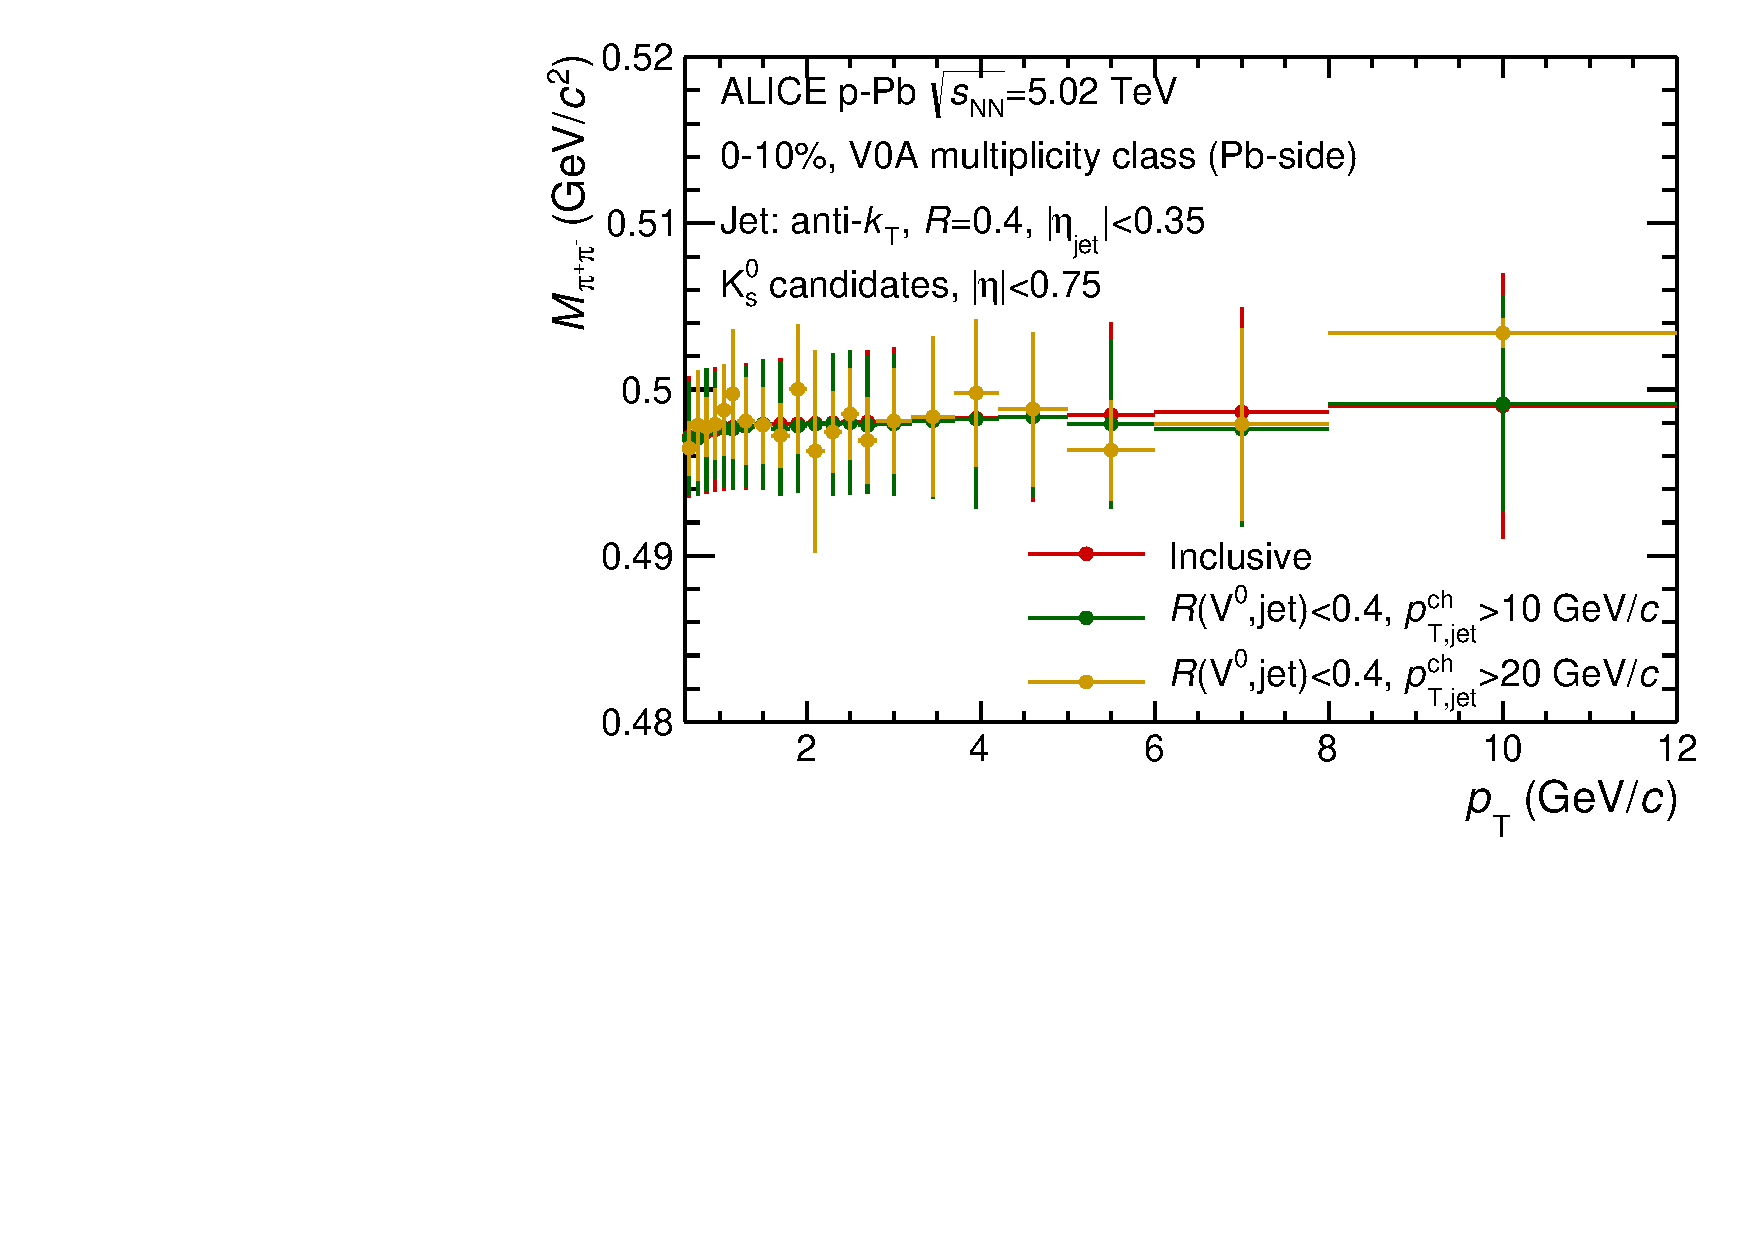
\includegraphics[width=.48\textwidth]{cFitInvM_Kshort}
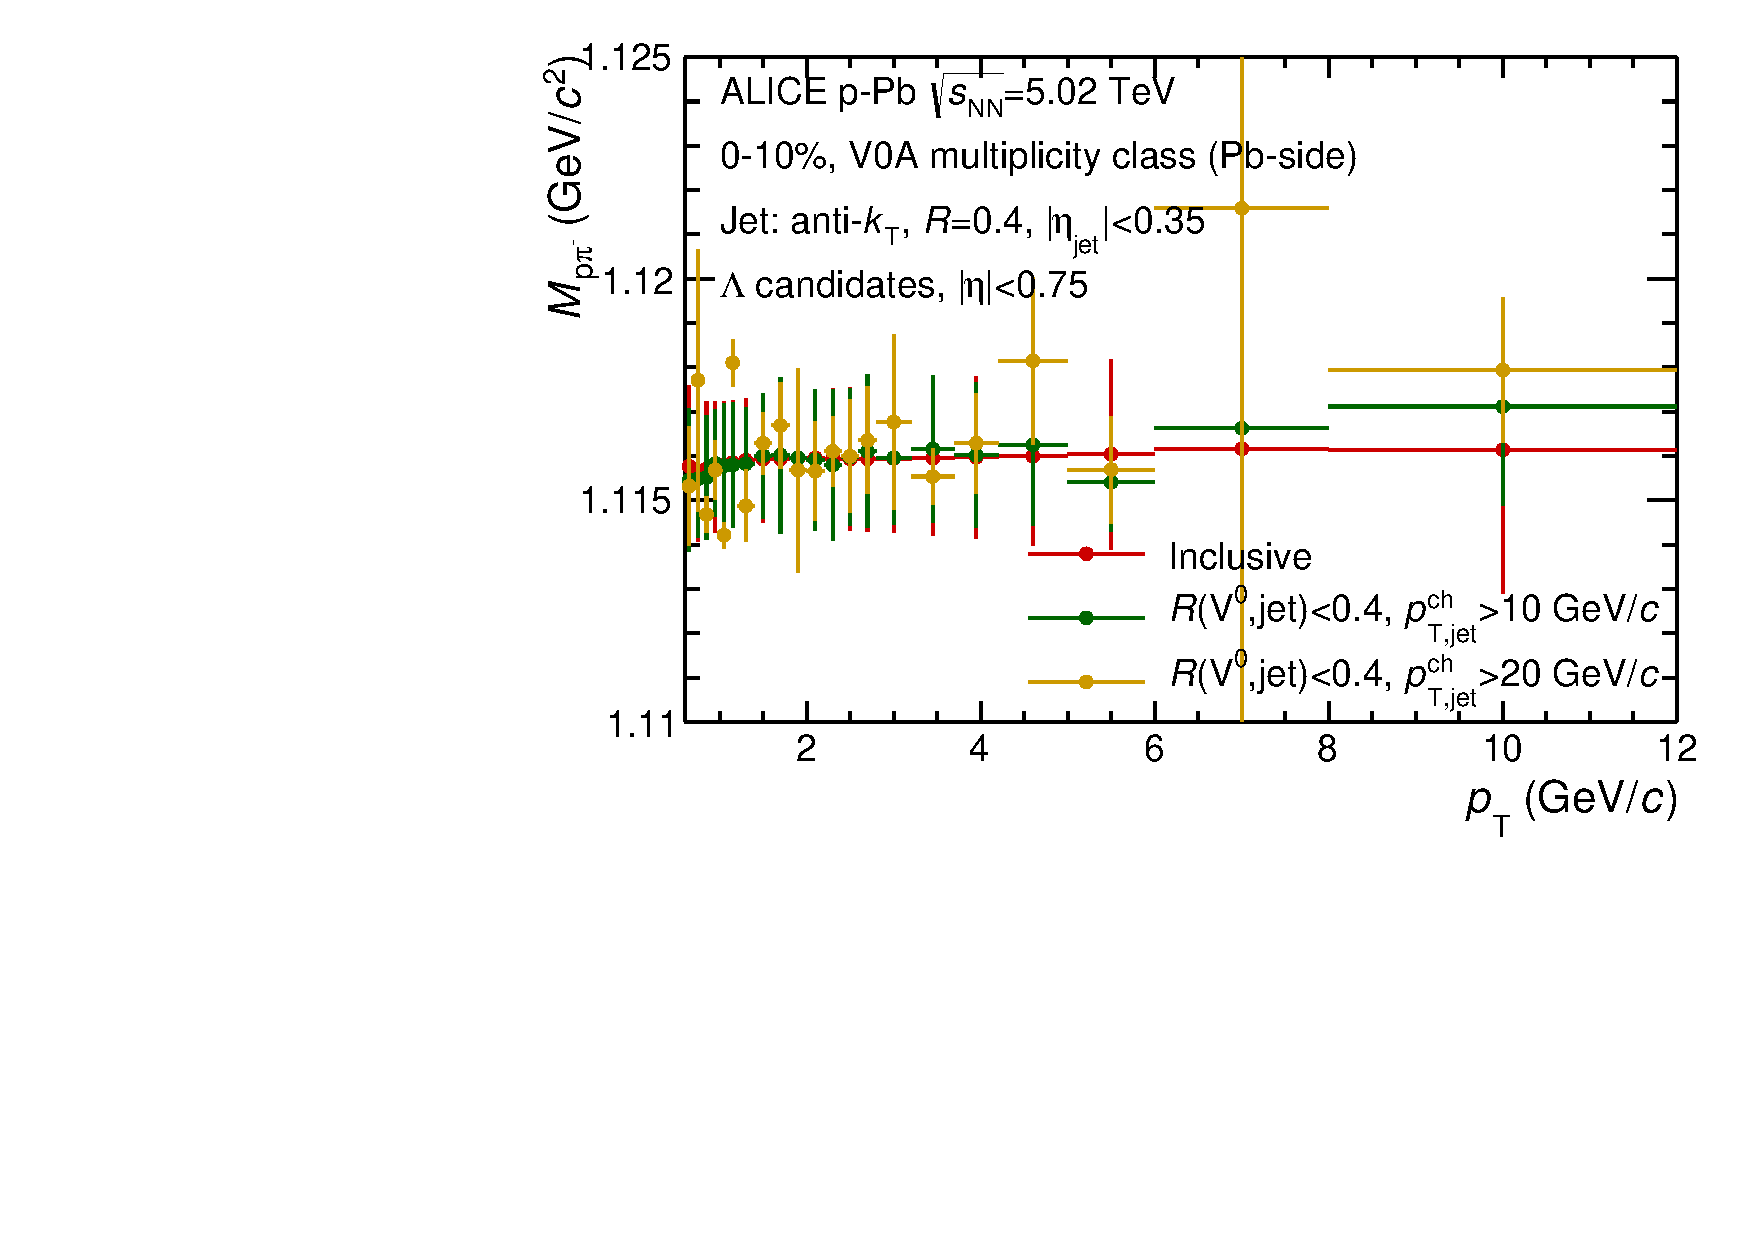
\includegraphics[width=.48\textwidth]{cFitInvM_Lambda}
\caption{The $\pT$-dependent mean of $\Vzero$ invariant mass distribution extracted by the Gaussian fit. The vertical error bar shows the width of the distribution.}
\label{fig:c05V0FitInvM}
\end{center}
\end{figure}

The contribution of $\Xi^{\pm}$ weak decays to the inclusive $\Lambda$ ($\AntiLa$) yield was corrected following a data-driven approach~\cite{Abelev:2013haa} using the measured $\Xi^{\pm}$ spectra as the inputs in a simulation of decay kinematics to evaluate the fraction of feed-down $\Lambda$ ($\AntiLa$).
The contribution from $\Xi^{0}$ decays was taken into account in the same way by assuming $\Xi^{-}(\Xi^{+})/\Xi^{0}=1$~\cite{Abelev:2013haa,Roesler:2000he,Skands:2010ak}.
The feed-down contribution for $\Lambda$ ($\AntiLa$) with JC selection was estimated based on the evaluated feed-down fraction of inclusive $\Lambda$ ($\AntiLa$) at high-$\pT$ and interpolated to the lower $\pT$ using \textsc{Pythia}\,8~\cite{Sjostrand:2007gs} Monte Carlo simulations.
\ask{-- Do we need more details?}

The acceptance and reconstruction efficiency was extracted from a Monte Carlo simulation based on \textsc{Dpmjet}\,3.05 event generator~\cite{Roesler:2000he} and GEANT\,3.21~\cite{Brun:1994aa} transport model for the detector (more details can be found in~\cite{Aamodt:2011zza}).
It has been shown that, the $\pT$ and $\eta$-dependent local efficiencies, $\epsilon(\pT,\eta)$, of $\Vzero$s in different selections are the same \ask{(is there a ref?)}.
To correct the $\pT$-differential yield, the $\pT$-dependent efficiency, $\epsilon(\pT)$, is given by integrating local efficiency over pseudo-rapidity acceptance weighted by $\Vzero$ distribution in data:
\begin{equation}\label{eq:c05EffiV0}
\epsilon(\pT)=\frac{\sum_{\hlab}n(\pT,\hlab)\epsilon(\pT,\hlab)}{\sum_{\hlab}n(\pT,\hlab)},
\end{equation}
where $n(\pT,\hlab)$ is the local yield of $\Vzero$s in data, it is estimated by the counts of $\Vzero$ candidate.
The bias from combinatory background is included in the statistic uncertainty of $\epsilon(\pT)$ and is propagated to the final results.
The efficiency of inclusive $\Vzero$s and JC $\Vzero$s with $R(\Vzero,{\rm jet})<0.4$ and $\pT[jet]>10~\GeVc$ are compared in figure~\ref{fig:c05EffiV0InJets}.
Since the yield of jets decreases when $\abs{\hlab}$ is increasing, a larger weight was assigned to JC $\Vzero$s around $\hlab=0$, where reaches the plateau of the maximum $\eta$-dependent efficiency, than inclusive $\Vzero$s in calculating $\epsilon(\pT)$.
It leads $\epsilon(\pT)$ of JC $\Vzero$s is systematically higher than inclusive $\Vzero$.
This effect is more significant at lower $\pT$.
\ask{-- Is this part clear? Some values will be cited in the text.}

\begin{figure}[t]
\begin{center}
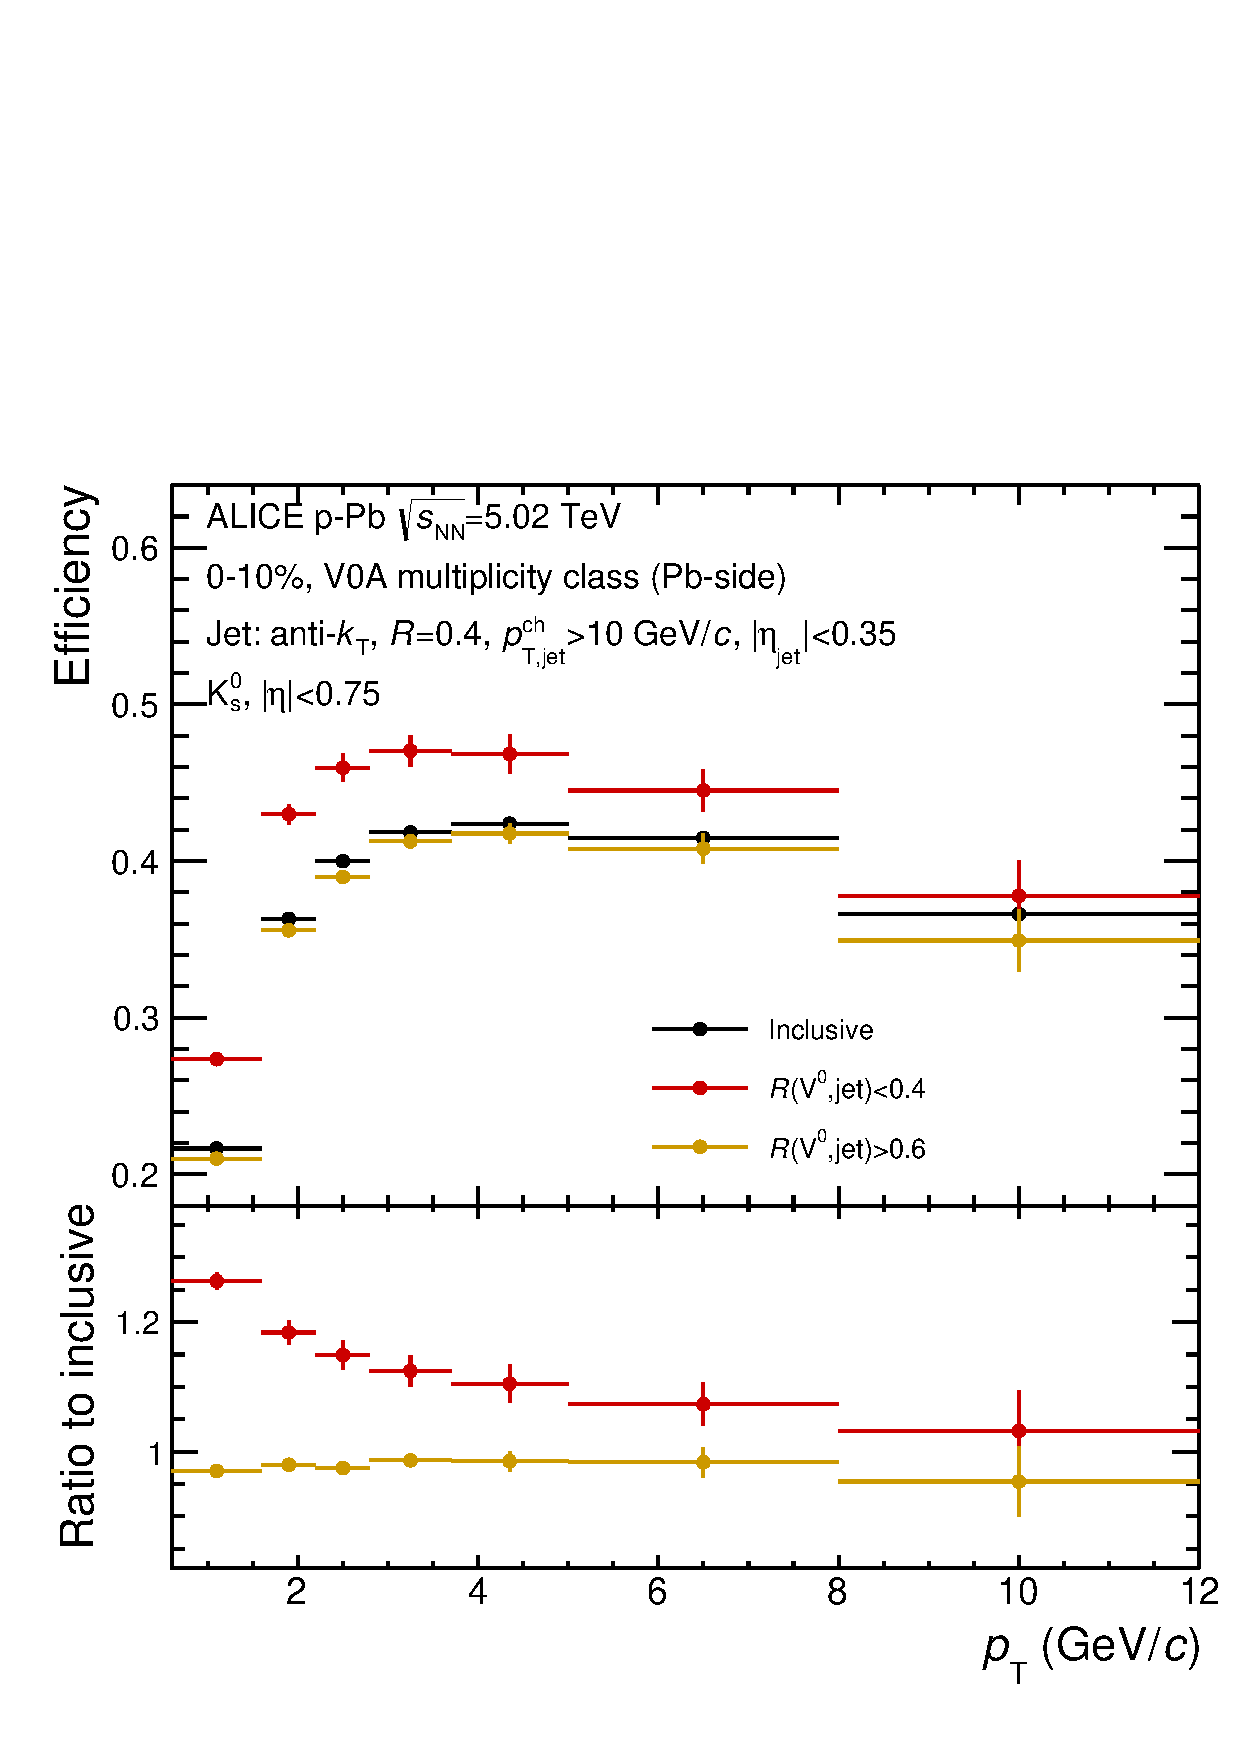
\includegraphics[width=.48\textwidth]{cEffiInJE_Kshort_JE_JR04_JC04_V0A_000_010}
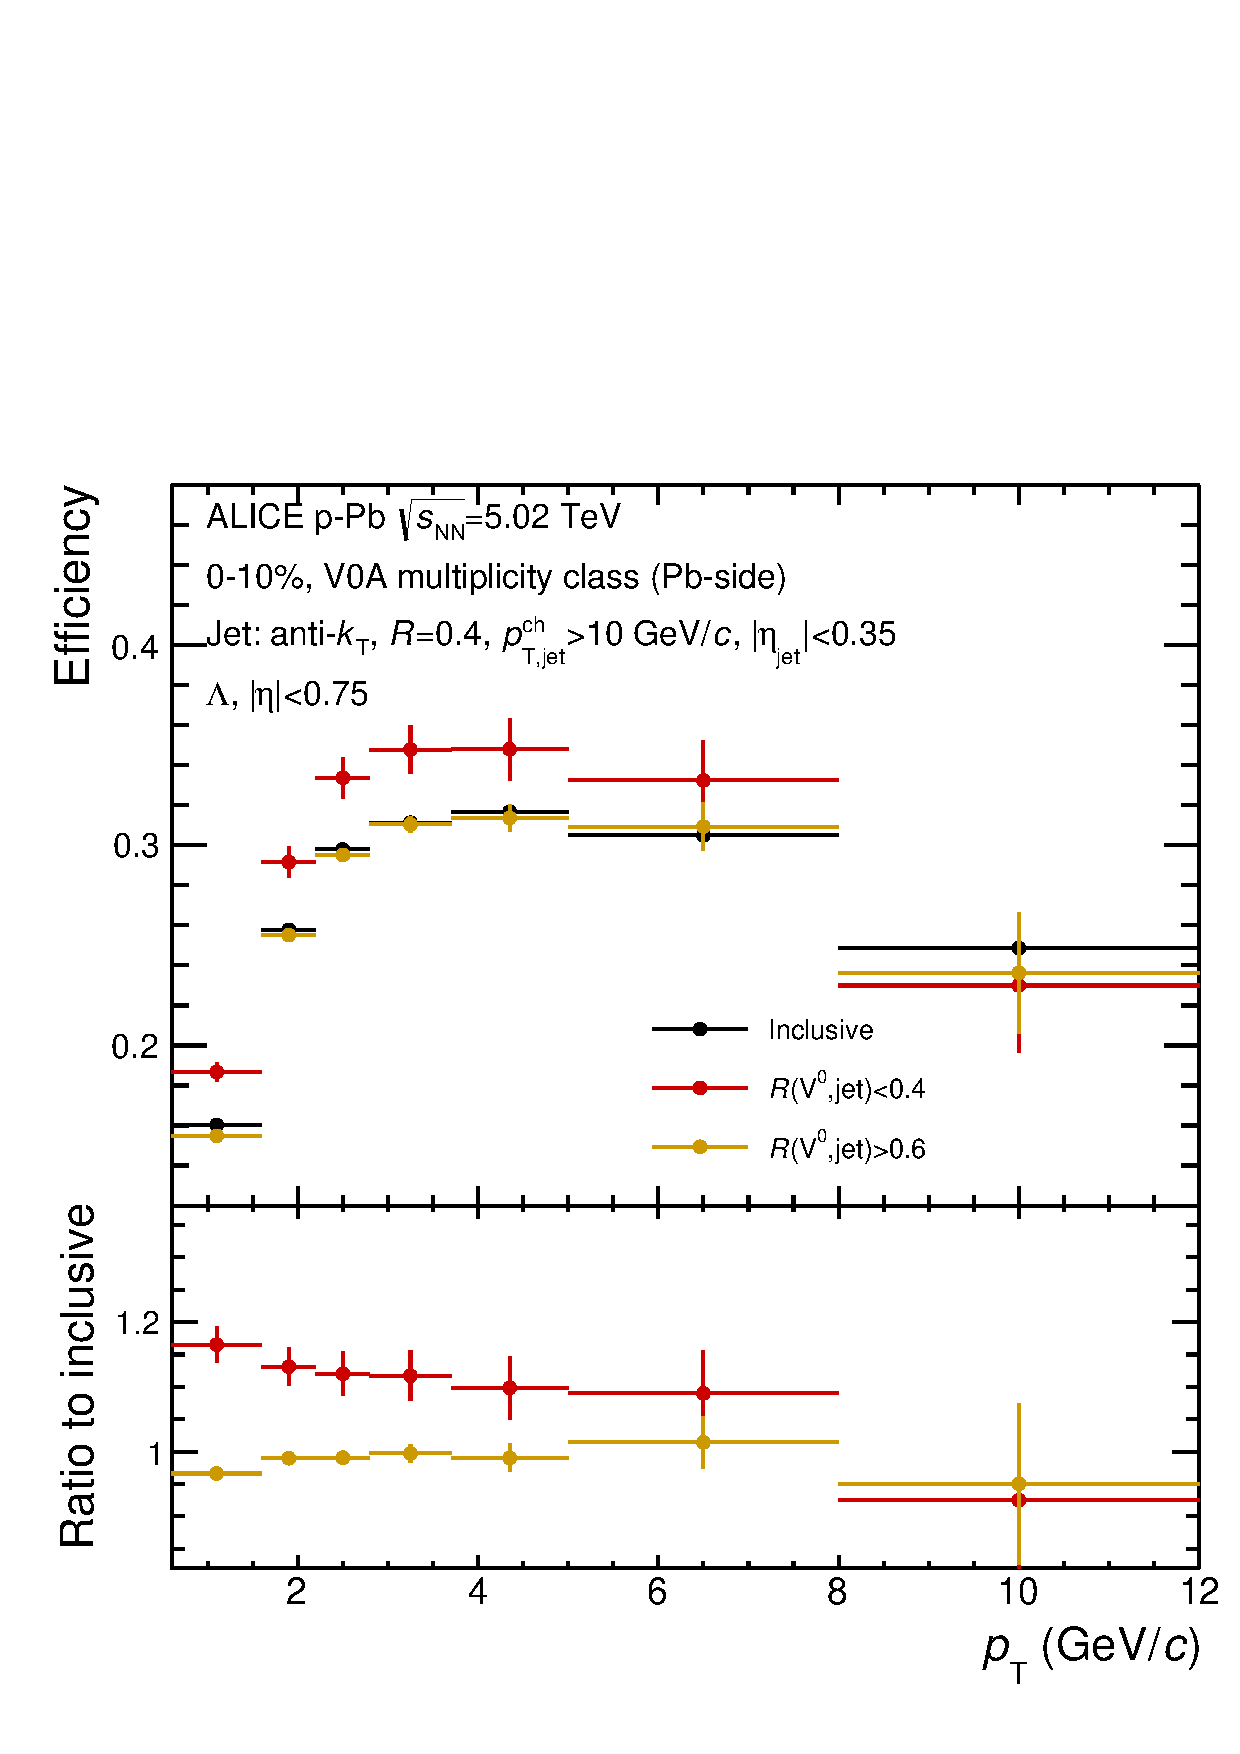
\includegraphics[width=.48\textwidth]{cEffiInJE_Lambda_JE_JR04_JC04_V0A_000_010}
\caption{Efficiency of inclusive $\Vzero$s as a function of $\pT$ \ask{(to be replaced by the MB ones)}.}
\label{fig:c05EffiV0InJets}
\end{center}
\end{figure}

To obtain the contribution from underlying event (UE $\Vzero$s, not associated to the hard scatterings) to the yield of JC $\Vzero$s, several estimators have been investigated.
\begin{itemize}
\item The OC selection: the $\Vzero$ candidates those were not matched to any selected jet with $R(\Vzero,{\rm jet})>R_{\rm cut}$.
\item The PC selection: the $\Vzero$ candidates found in the cones in the perpendicular directions of the selected jets \ask{(Add the PC definition explicitly? -- four PC cones are used)}.
\item The NJ selection: the $\Vzero$ candidates found in events those do not contain any jet with $\pT[jet]>5~\GeVc$.
\end{itemize}
The yields of different UE selections are extracted via the same approach as the JC $\Vzero$s.
The efficiency of OC $\Vzero$s with $R_{\rm cut}=0.6$ and $\pT[jet]>10~\GeVc$ is compared to those of inclusive $\Vzero$s and JC $\Vzero$s in figure~\ref{fig:c05EffiV0InJets}.
The efficiency of OC $\Vzero$s is similar to the inclusive $\Vzero$s and only a few precent lower than the inclusive one at low $\pT$.

\begin{figure}[t]
\begin{center}
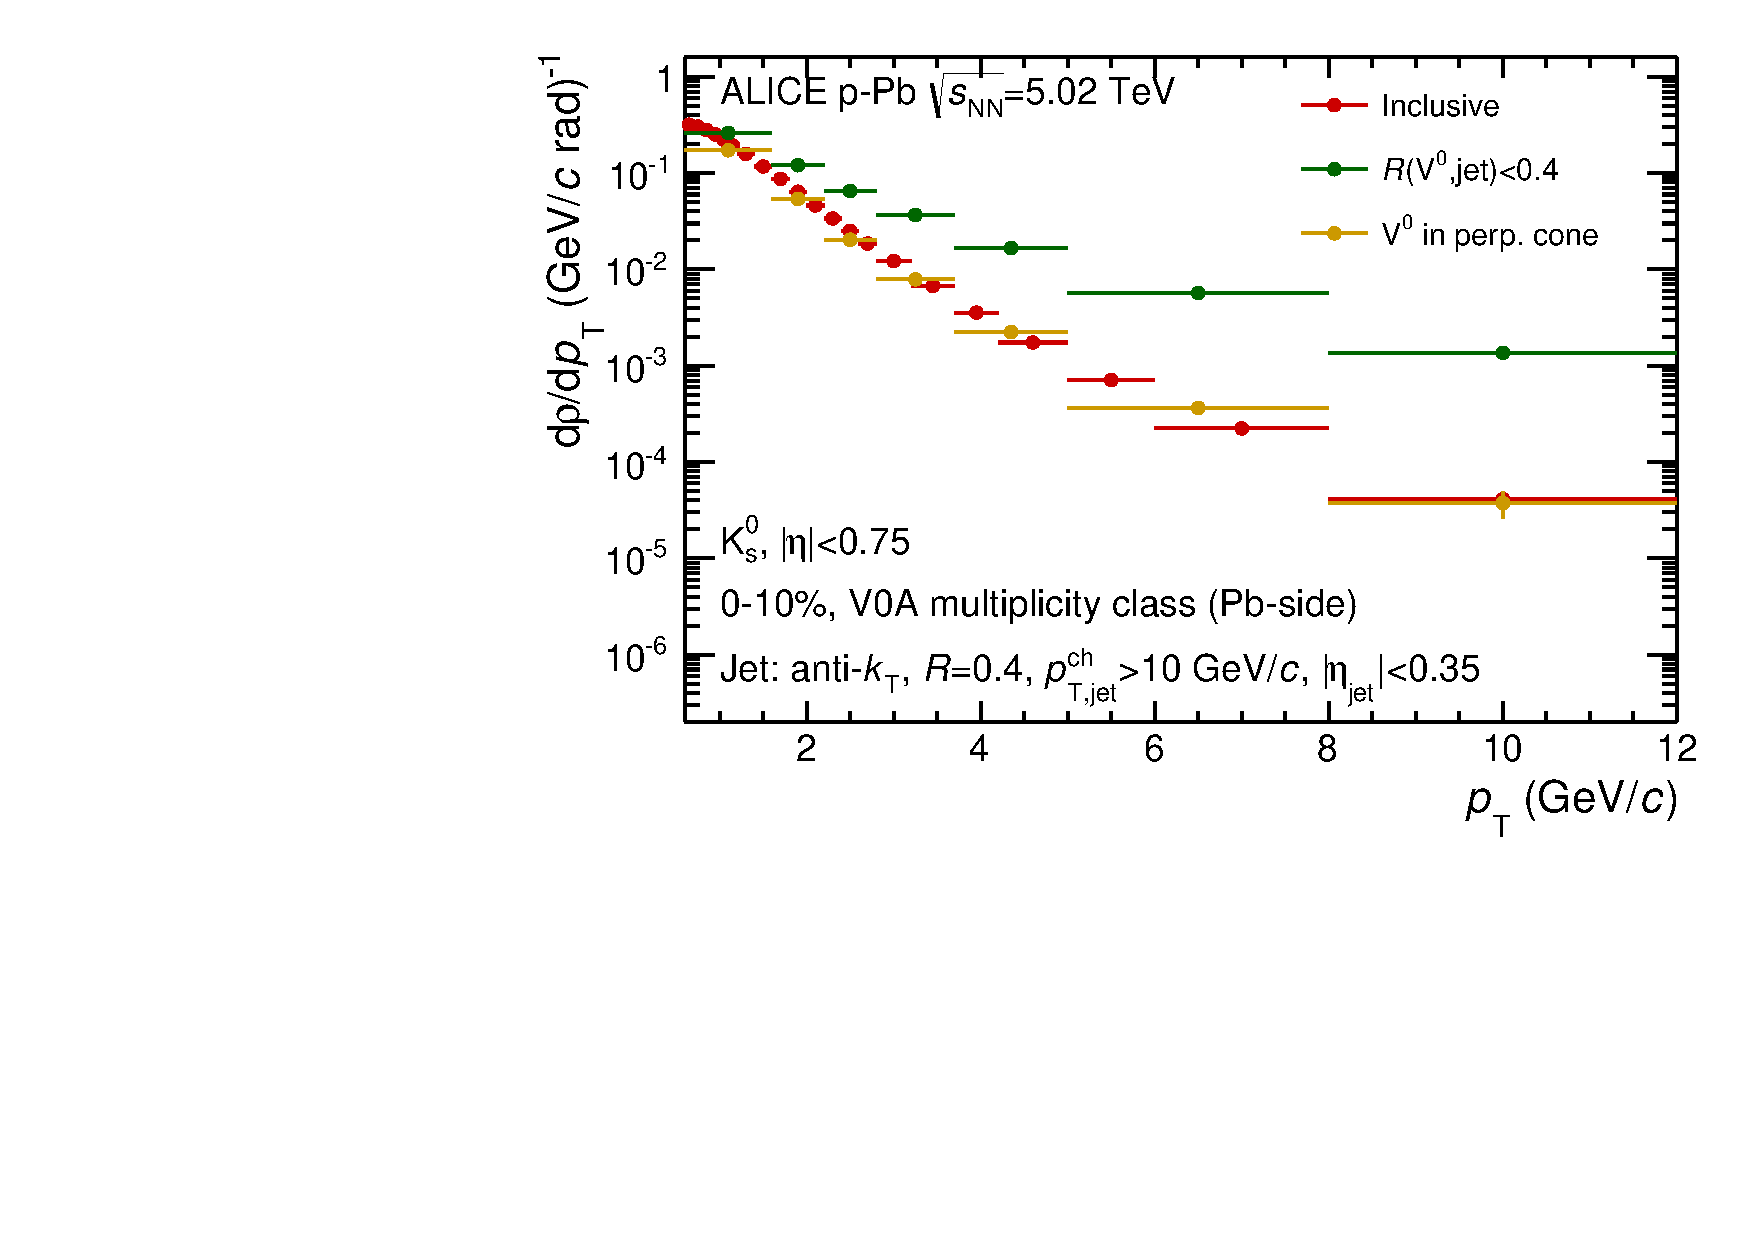
\includegraphics[width=.48\textwidth]{cRho_Kshort_JE_JR04_JC04_V0A_000_010}
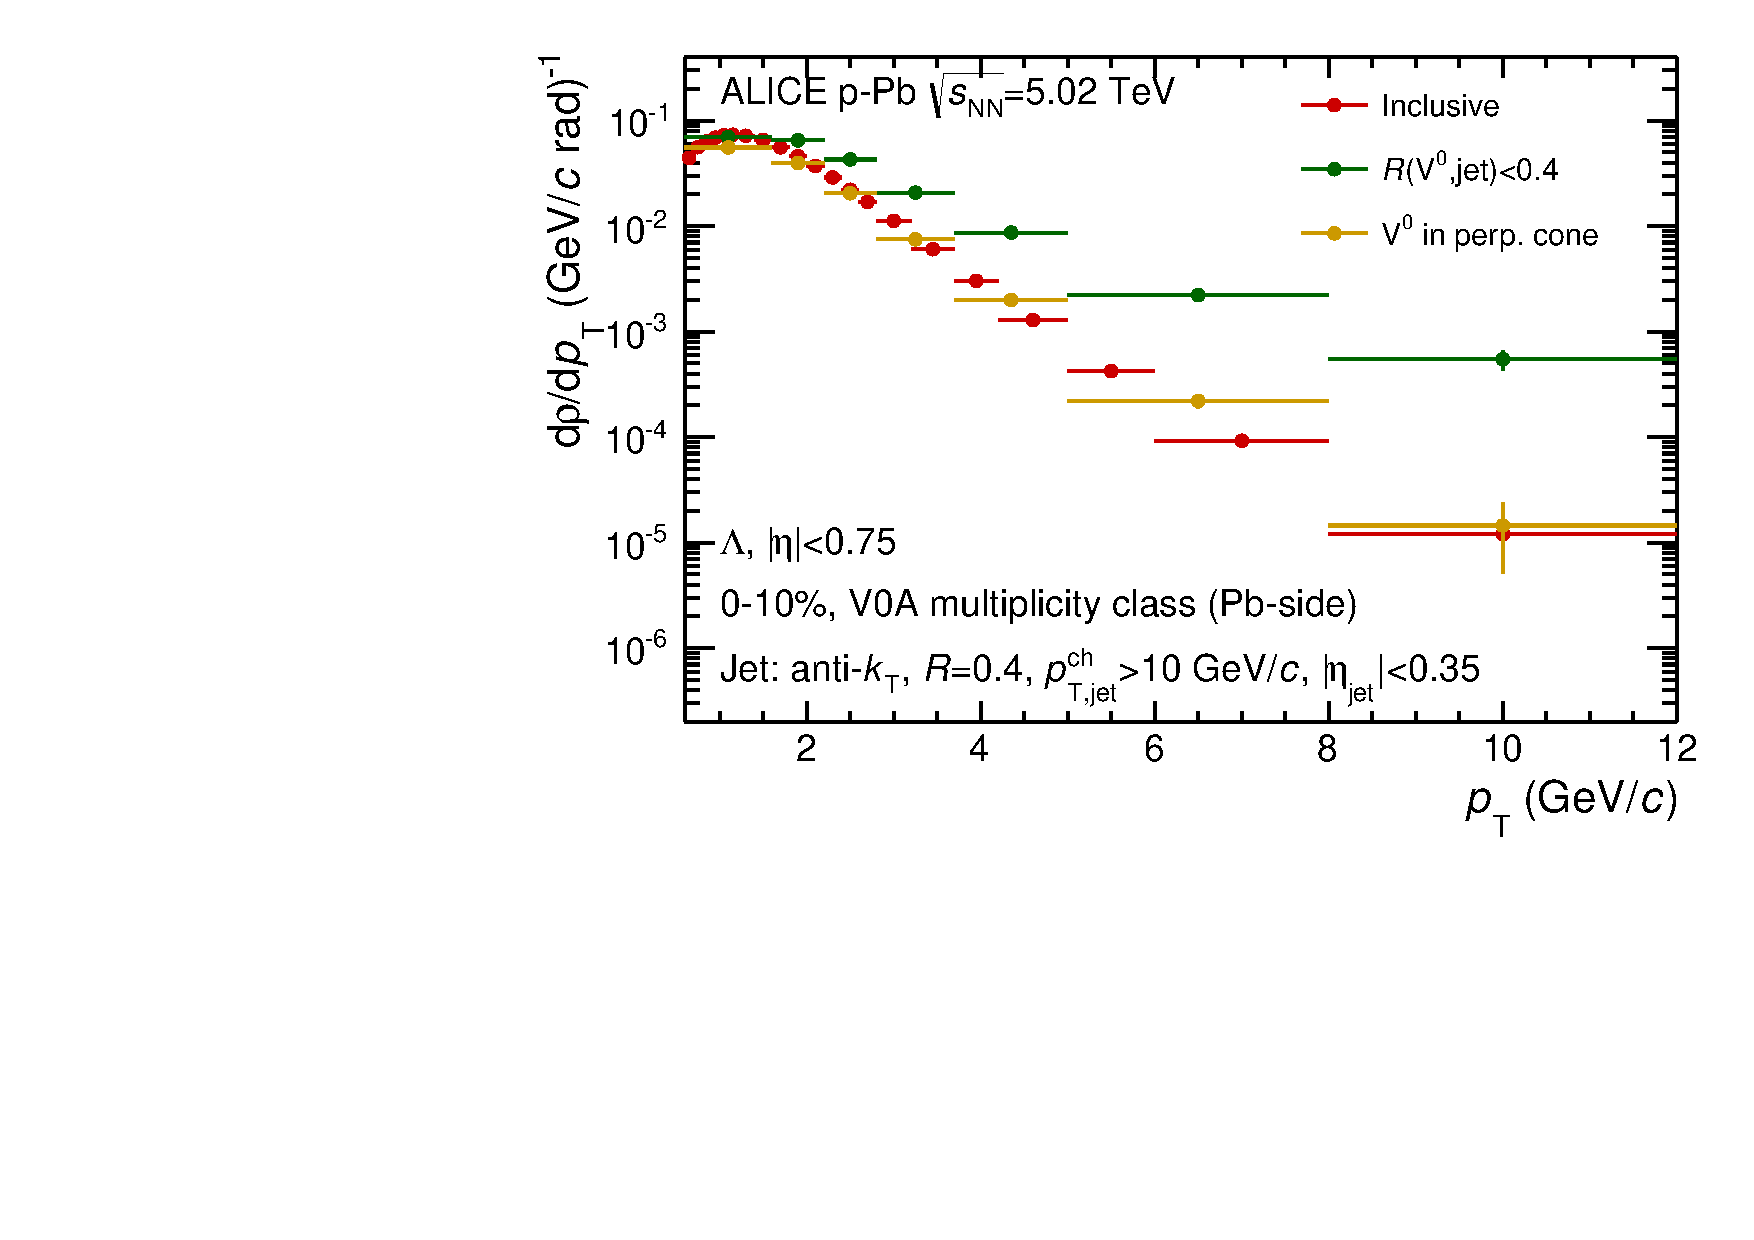
\includegraphics[width=.48\textwidth]{cRho_Lambda_JE_JR04_JC04_V0A_000_010}
\caption{$\pT$-differential density of $\Vzero$s in different selections \ask{(to be replaced by the MB ones)}.}
\label{fig:c05SpecV0s}
\end{center}
\end{figure}

Finally, to subtract the UE contribution from the JC selection, the efficiency corrected spectra of JC $\Vzero$s and UE $\Vzero$s have been normalized to the density per unit area,
\begin{equation}
\frac{\dd\rho_{\Vzero}}{\dd\pT}=\frac{1}{N_{\rm ev}}~\frac{1}{\avg{A_{\Vzero}}}~\frac{\dd N_{\Vzero}}{\dd\pT},
\end{equation}
where is $\avg{A_{\Vzero}}$ is the average acceptance for a given $\Vzero$ selection in $\hlab$--$\varphi$ plane calculated on a event-by-event basis.
Figure~\ref{fig:c05SpecV0s} shows the $\pT$-differential density distribution of inclusive $\Vzero$s and the JC and PC selections.
The $\pT$-differential density distribution of JC $\Vzero$s is much harder than those of inclusive $\Vzero$s and UE $\Vzero$s.
The density of $\Vzero$s associated to the hard scatterings, therefore, is obtained subtracting the density of UE $\Vzero$s from the JC selections.
\ask{More statements are needed -- (?)}

\subsection{Systematic uncertainty}
\label{sec:Syst}

\begin{figure}[t]
\begin{center}
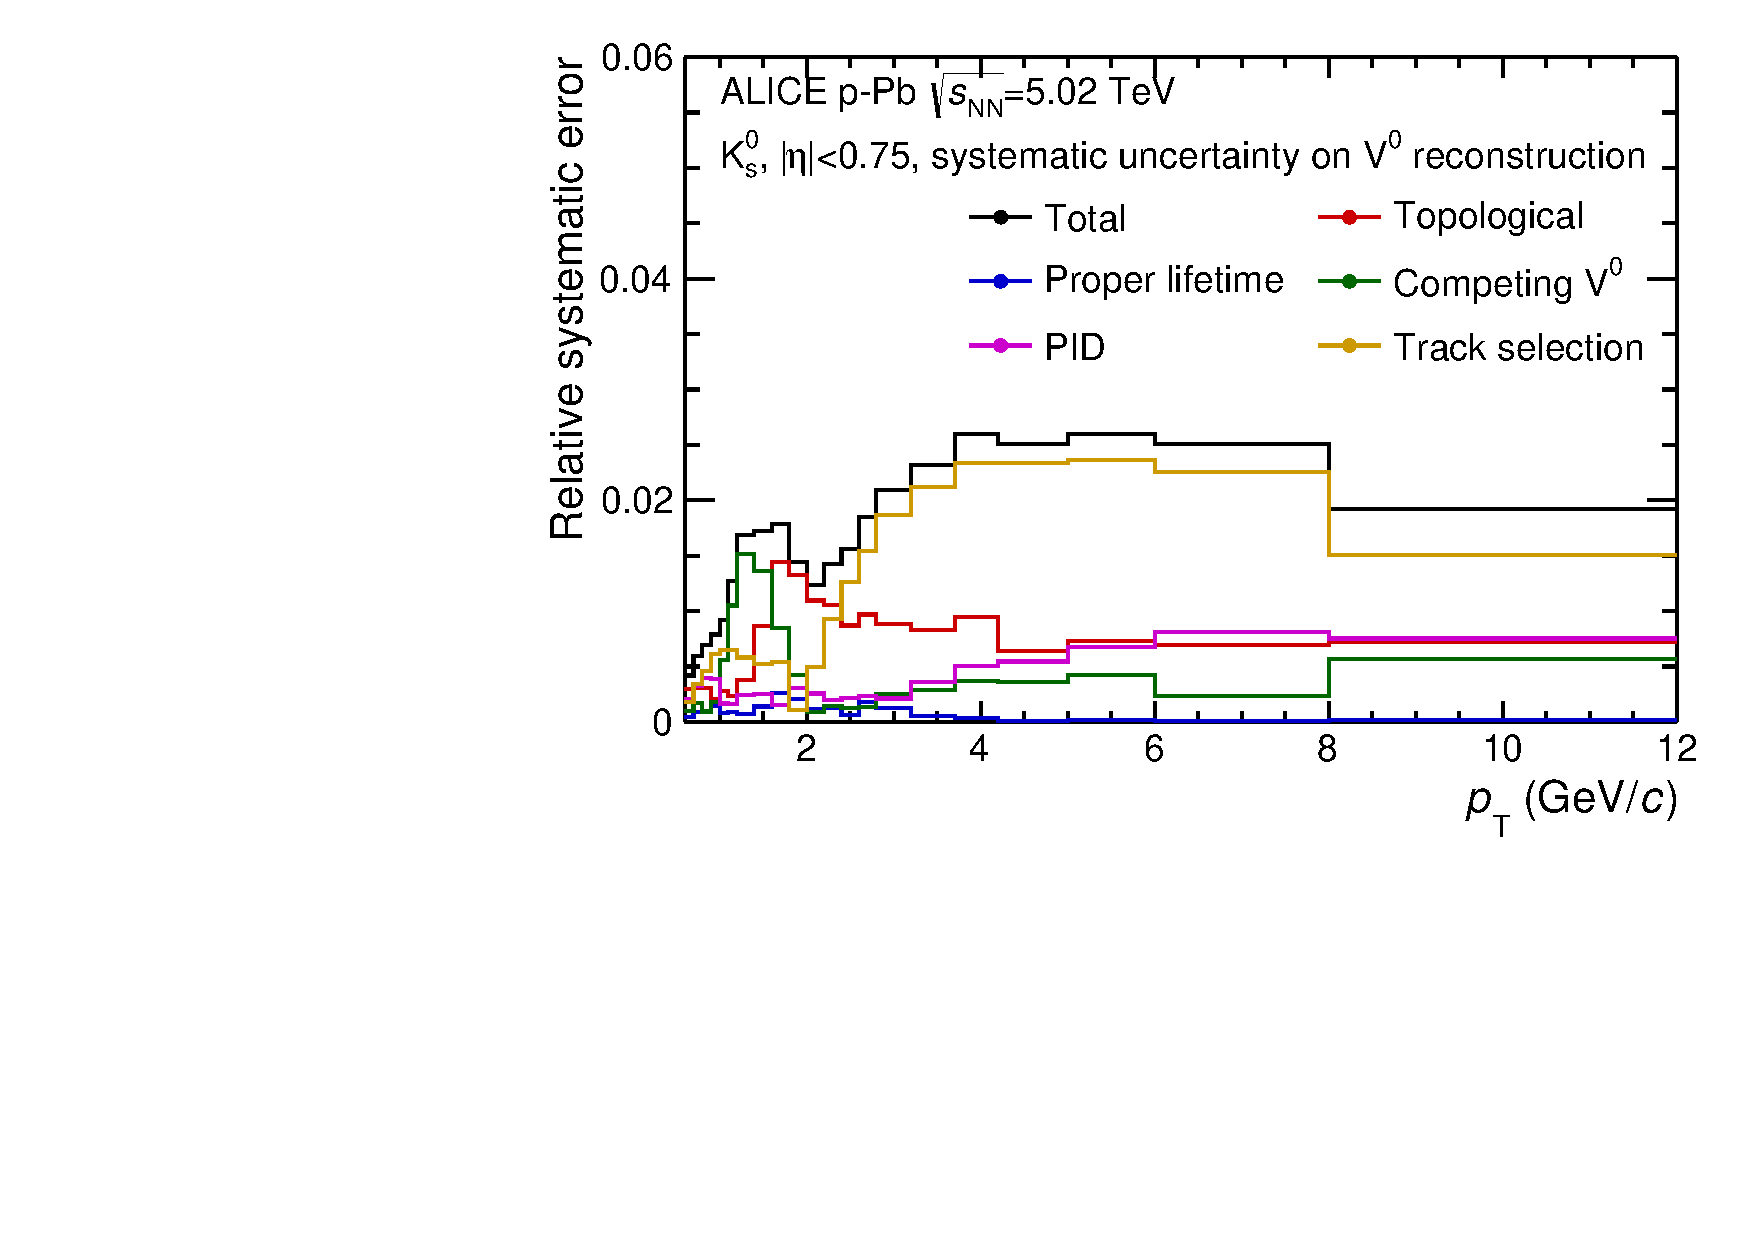
\includegraphics[width=.32\textwidth]{cSystIncl_Kshort}
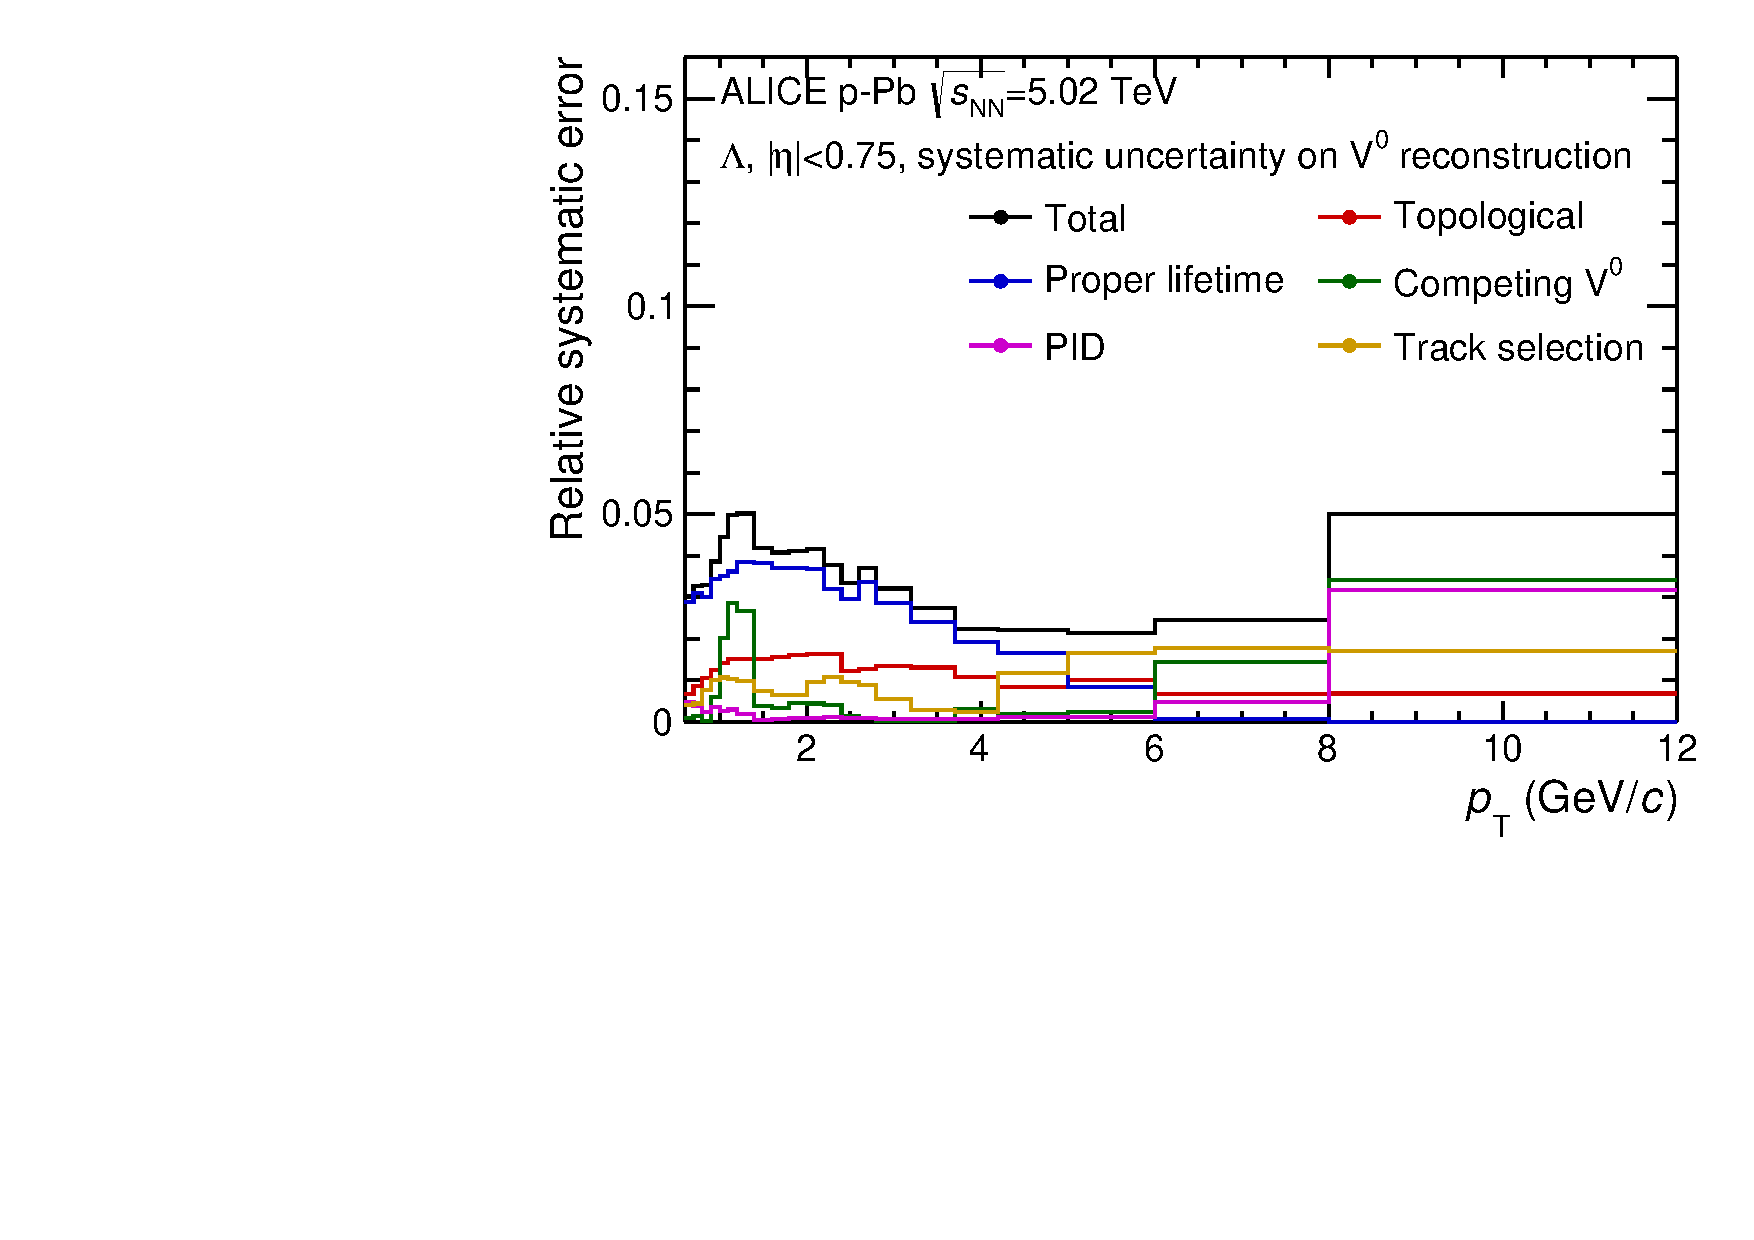
\includegraphics[width=.32\textwidth]{cSystIncl_Lambda}
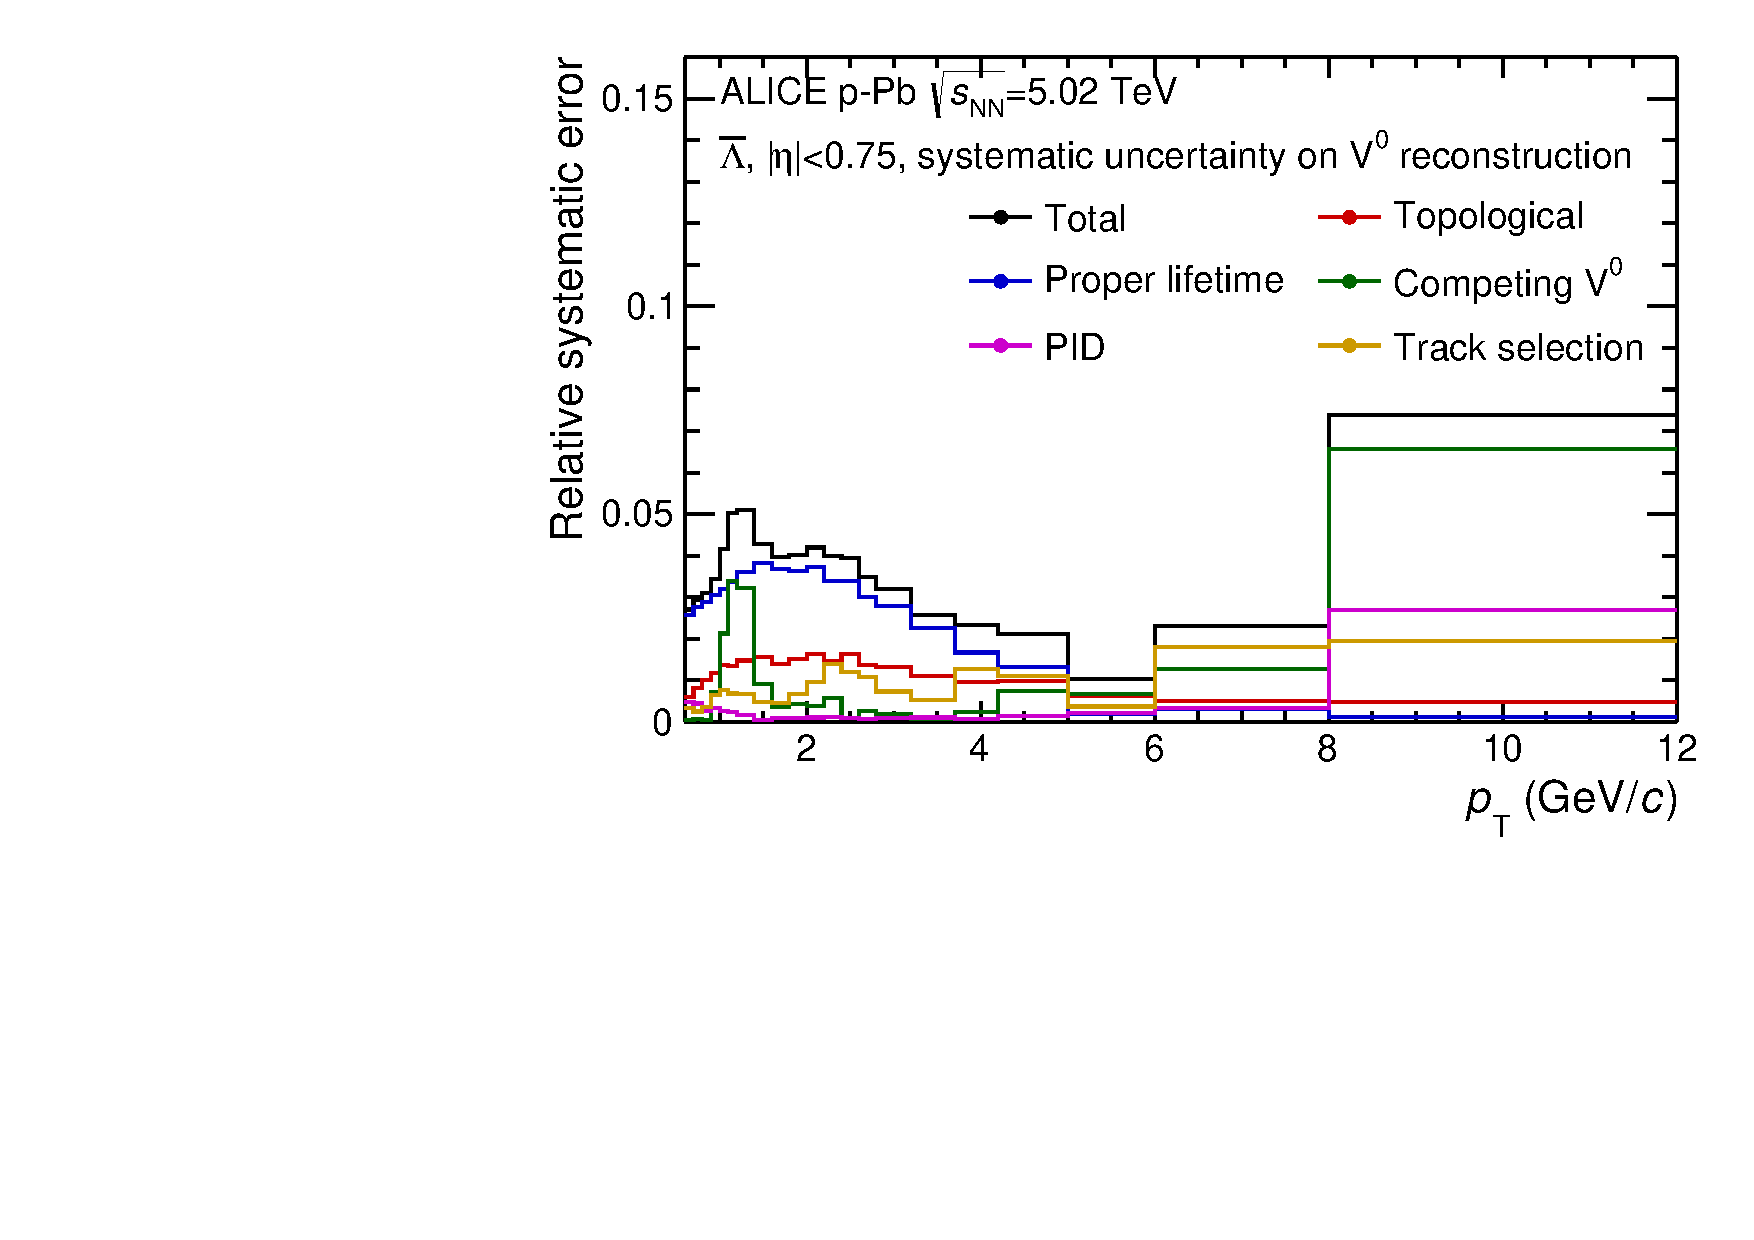
\includegraphics[width=.32\textwidth]{cSystIncl_AntiLa}
\caption{Systematic uncertainty of inclusive $\Vzero$s -- uncorrelated with statistics.}
\label{fig:c06SystInclV0s}
\end{center}
\end{figure}

\begin{figure}[t]
\begin{center}
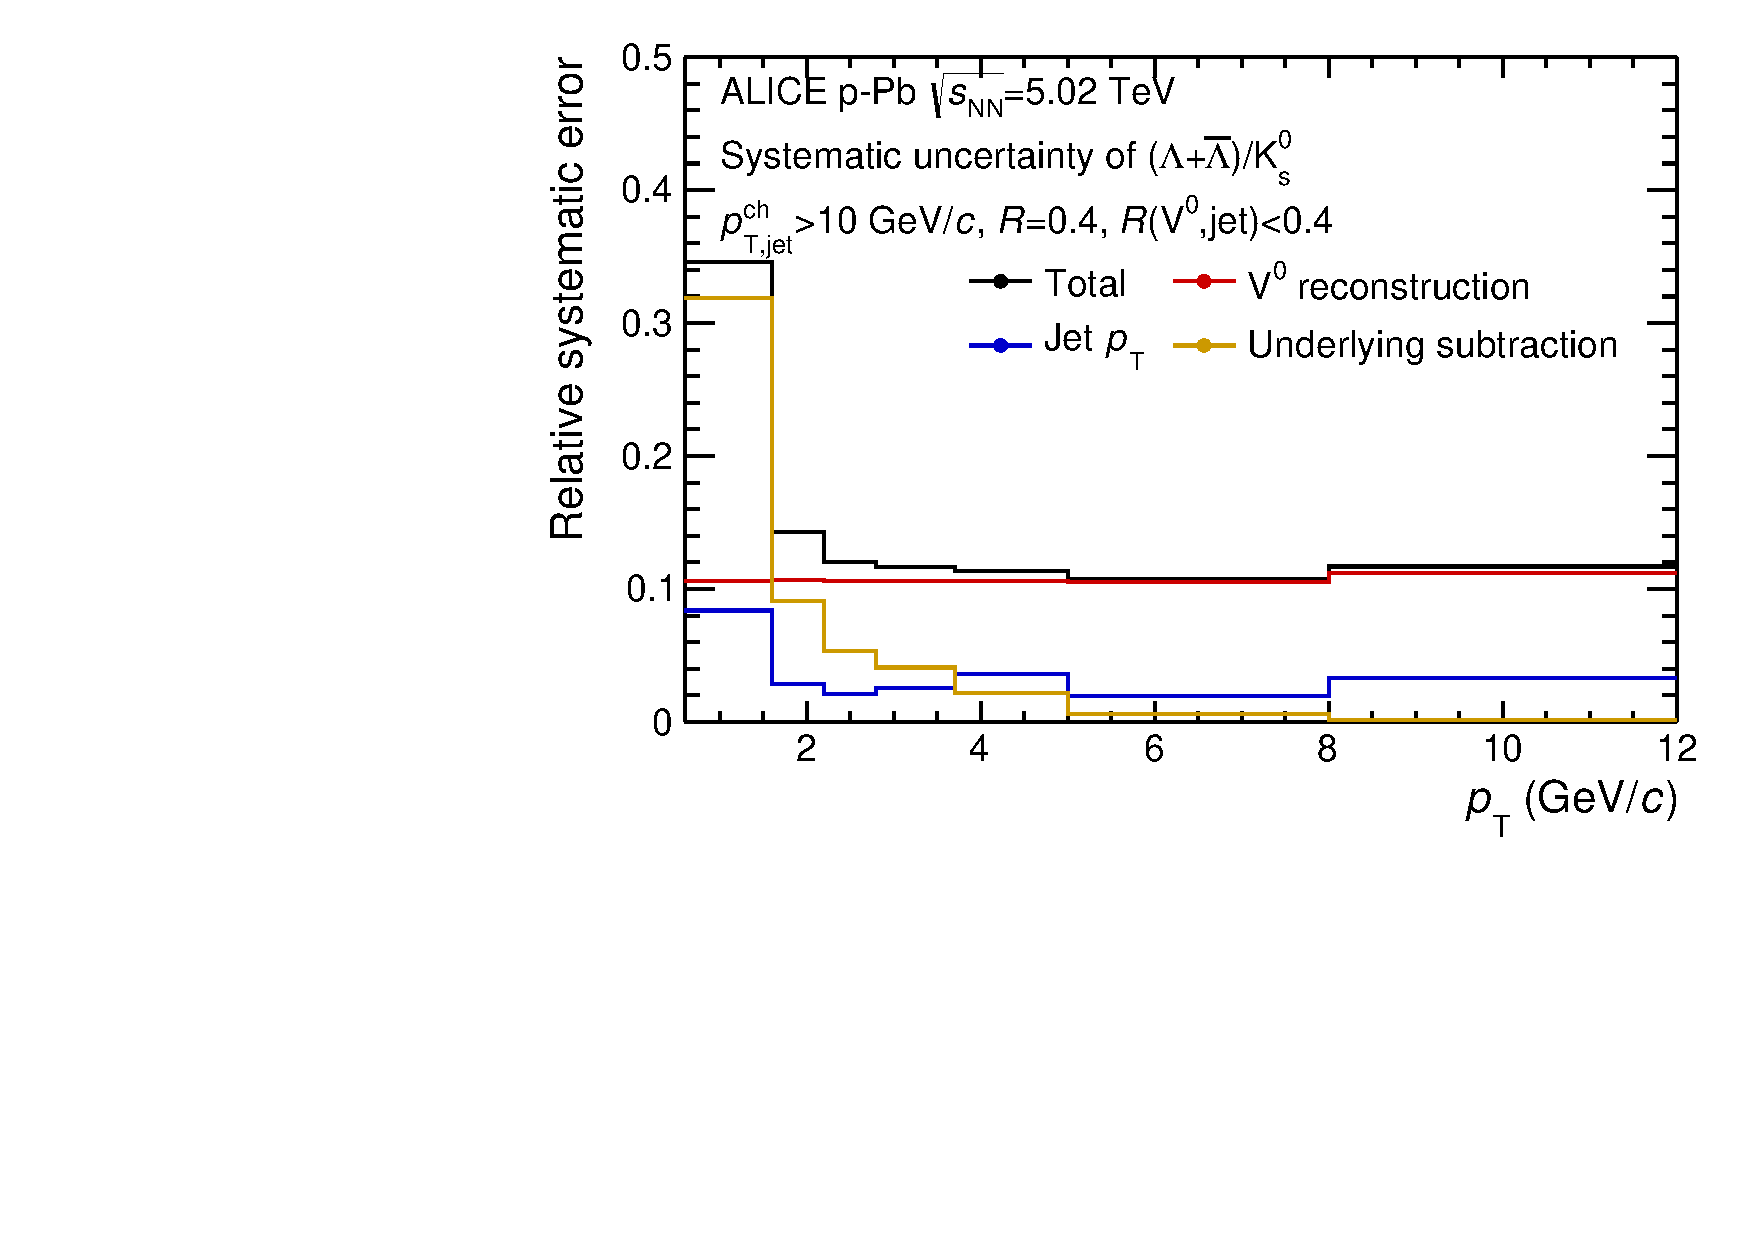
\includegraphics[width=.48\textwidth]{cSystInJE_RatioV_Ptj10}
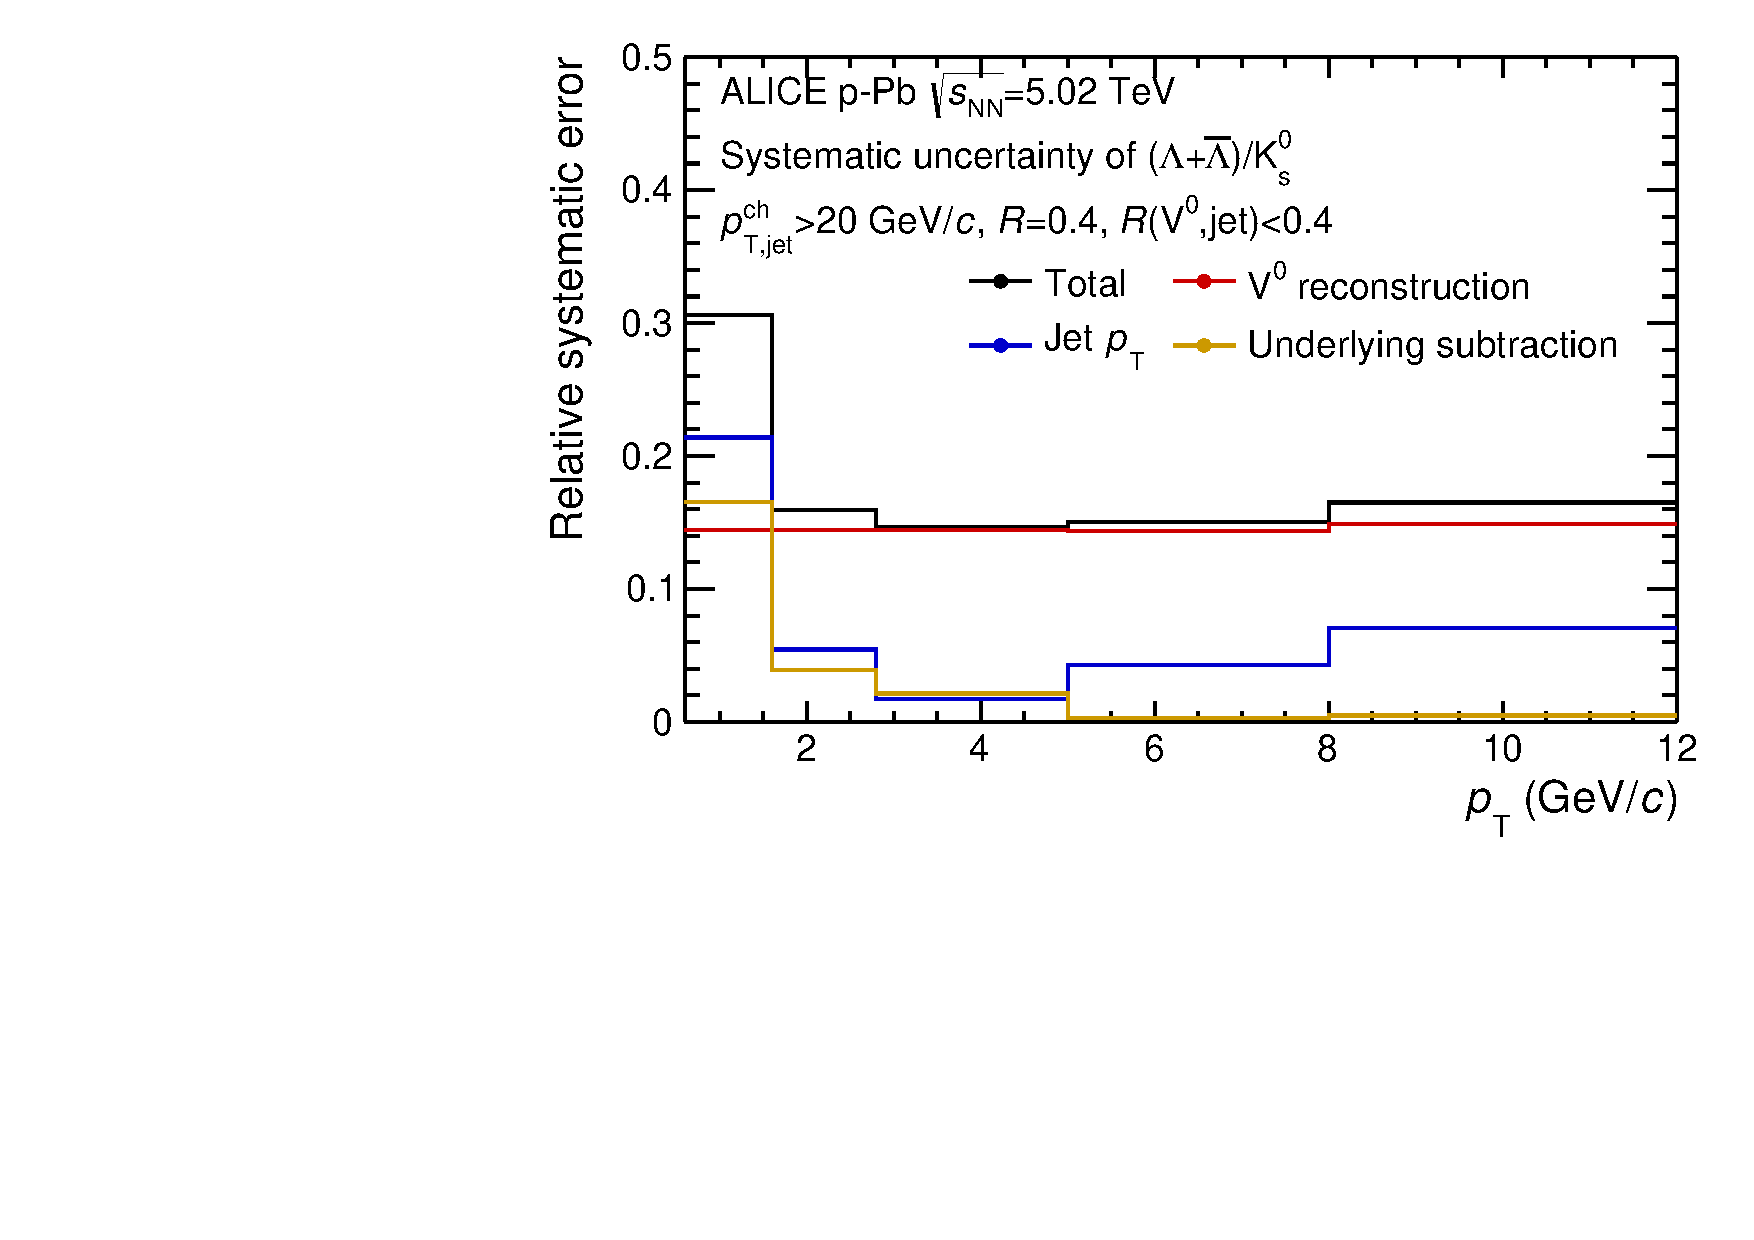
\includegraphics[width=.48\textwidth]{cSystInJE_RatioV_Ptj20}
\caption{Systematic uncertainty of $\Vzero$s in jets -- correlated with statistics.}
\label{fig:c06SystV0InJets}
\end{center}
\end{figure}

The systematic uncertainty includes two catalogs.

One is independent on different $\Vzero$ selections and is evaluated using inclusive $\Vzero$s.
The knowledge of detector materials resulting a $4\%$ uncertainty~\cite{Abelev:2013haa}.
Track and topology selections, up to $3\%$ ($5\%$) for $\Kshort$ ($\Lambda$ and $\AntiLa$) depend on $\pT$ (see~\cite{Abelev:2013xaa} for the details).
The systematic uncertainty on feed-down correction for $\Lambda$ and $\AntiLa$ was used the spread of the feed-down fractions determined for different event multiplicity ranges with respect to the minimum bias events is $5\%$ ($7\%$) in $\pT<3.7~\GeVc$ ($<3.7~\GeVc$)~\cite{Abelev:2013haa}.
For the JC selection, an extra $5\%$ \ask{(to be checked)} uncertainty was added in $\pT<6~\GeVc$ for the discrepancy between \textsc{Pythia} interpolations and the values for inclusive $\Lambda$ and $\AntiLa$.

\begin{table}[t]
\centering 
\begin{tabular*}{\linewidth}{@{\extracolsep{\fill}}lccc}
\hline
&&&\\[-0.7em]
 & $\Kshort$ & \multicolumn{2}{c}{$\Lambda$($\AntiLa$)}\\[0.3em]
\hline
&&&\\[-0.7em]
Proper lifetime & 2\% & \multicolumn{2}{c}{2\%} \\[0.3em]
Material budget & 4\% & \multicolumn{2}{c}{4\%} \\[0.3em]
Track selection  & 4\% & \multicolumn{2}{c}{4\%} \\[0.3em]
TPC PID & 1\% & \multicolumn{2}{c}{1\%} \\[0.3em]
Multiplicity & \multirow{2}{*}{2\%} & \multicolumn{2}{c}{\multirow{2}{*}{2\%}} \\
dependence & & \\[0.3em]
\hline
\hline
&&&\\[-0.7em]
\pT\ (\GeVc)  &  & $<$ 3.7 & $>$ 3.7\\[0.3em]
\hline
&&&\\[-0.7em]
Feed-down  &  & \multirow{2}{*}{5\%} & \multirow{2}{*}{7\%}\\
correction & & &\\[0.3em]
    \hline
    \hline
    &&&\\[-0.7em]
\pT\ (\GeVc)  &  & $<$ 3.7 & $>$ 3.7\\[0.3em]
    \hline
    &&&\\[-0.7em]
    Total & 6.5\% & 8\% & 9.5\% \\[0.3em]
\hline
\end{tabular*}
\caption{Main sources of systematic uncertainty for the $\Kshort$ and $\Lambda$($\AntiLa$).} \label{tab:v0syst}
\end{table}

In another catalog, the uncertainty on signal extraction, is depend on the various of $\Vzero$ selections.
As shown in section~\ref{sec:V0Reco}, to subtract the combinatory background via the bin counting approach, the signal region and sidebands are defined in $[-N\sigma,N\sigma]$ and, $[-2N\sigma,-N\sigma]$ and $[N\sigma,2N\sigma]$, respectively, where $\sigma$ is the $\pT$-dependent mass resolution, nominal $N=6$.
The $\pT$-dependent uncertainty on signal extraction is estimated by choosing the maximal deviation between varied $N$ in $4$, $5$ and $7$ and nominal spectra values obtained in each $\pT$ bin.
Since the bin counting fit is sensitive the statistic of $\Vzero$ candidates, this uncertainty is evaluated for each individual $\Vzero$ selection. \ask{-- Cite values, table or figure?}

There are two additional uncertainty sources for $\Vzero$s associated to the hard scatterings: the jet $\pT$ resolution and underlying event subtraction.
The applied jet $\pT$ threshold was smeared by local background fluctuations and detector response and, resulted a $\sim 20\%$ resolution independent on jet $\pT$~\cite{Adam:2015hoa}.
The analysis was repeated with varying the jet $\pT$ threshold within $20\%$\footnote{$e.g.$ for $\pT[jet]>10~\GeVc$ ($20~\GeVc$), the analysis was repeated in $\pT[jet]>8~\GeVc$ ($16~\GeVc$) and $\pT[jet]>12~\GeVc$ ($24~\GeVc$).} to evaluate the uncertainty on jet $\pT$ resolution.
For the underlying event subtraction, the PC selection was used as the default underlying event estimator, while the uncertainty was given using the OC with $R_{\rm cut}=0.6$ and NJ selections.
Each of these uncertainty source was evaluated as the $\pT$-dependent standard deviation between varied and nominal $\pT$-spectra values in each bin.
They were added in quadrature together with other uncertainties to yield the overall systematic uncertainty on the $\pT$ spectra.
Since these uncertainties are correlated for the $\Kshort$ and $\Lambda$ ($\AntiLa$) spectra and do partly cancel in the $\Lambda/\Kshort$ ratios.
In this case, they were evaluated by dividing $\Lambda$ ($\AntiLa$) and $\Kshort$ spectra obtained with the same selection variations.


\section{Results}
\label{sec:Results}

\subsection{$\pT$ yields}

\begin{itemize}
	\item yields in JC, OC, PC, NJ in minimum bias (+ inclusive - from the published paper)
	\item yields in JC, OC, PC, NJ in ``centrality'' bins
	\item ratio of the ``centrality'' bins to minimum bias \ask{NEW FIGURE! + discussion}
\end{itemize}

\ask{all above for V0 and ZNA - better into an appendix... (?); show the ``density'' plots?}

\ask{The yield are (also $\rho$ are shown in the previous sections. Will we only focus on the L/K ratio in this section?)}

\subsection{L/K ratios}

\begin{itemize}
	\item ratios in JC, OC, PC, NJ in minimum bias (+ inclusive from the published paper)
	\item ratios in JC, OC, PC, NJ in ``centrality'' bins
	\item ratio of the ``centrality'' bins to minimum bias \ask{NEW FIGURE! + discussion}
\end{itemize}


\begin{figure}[t]
\begin{center}
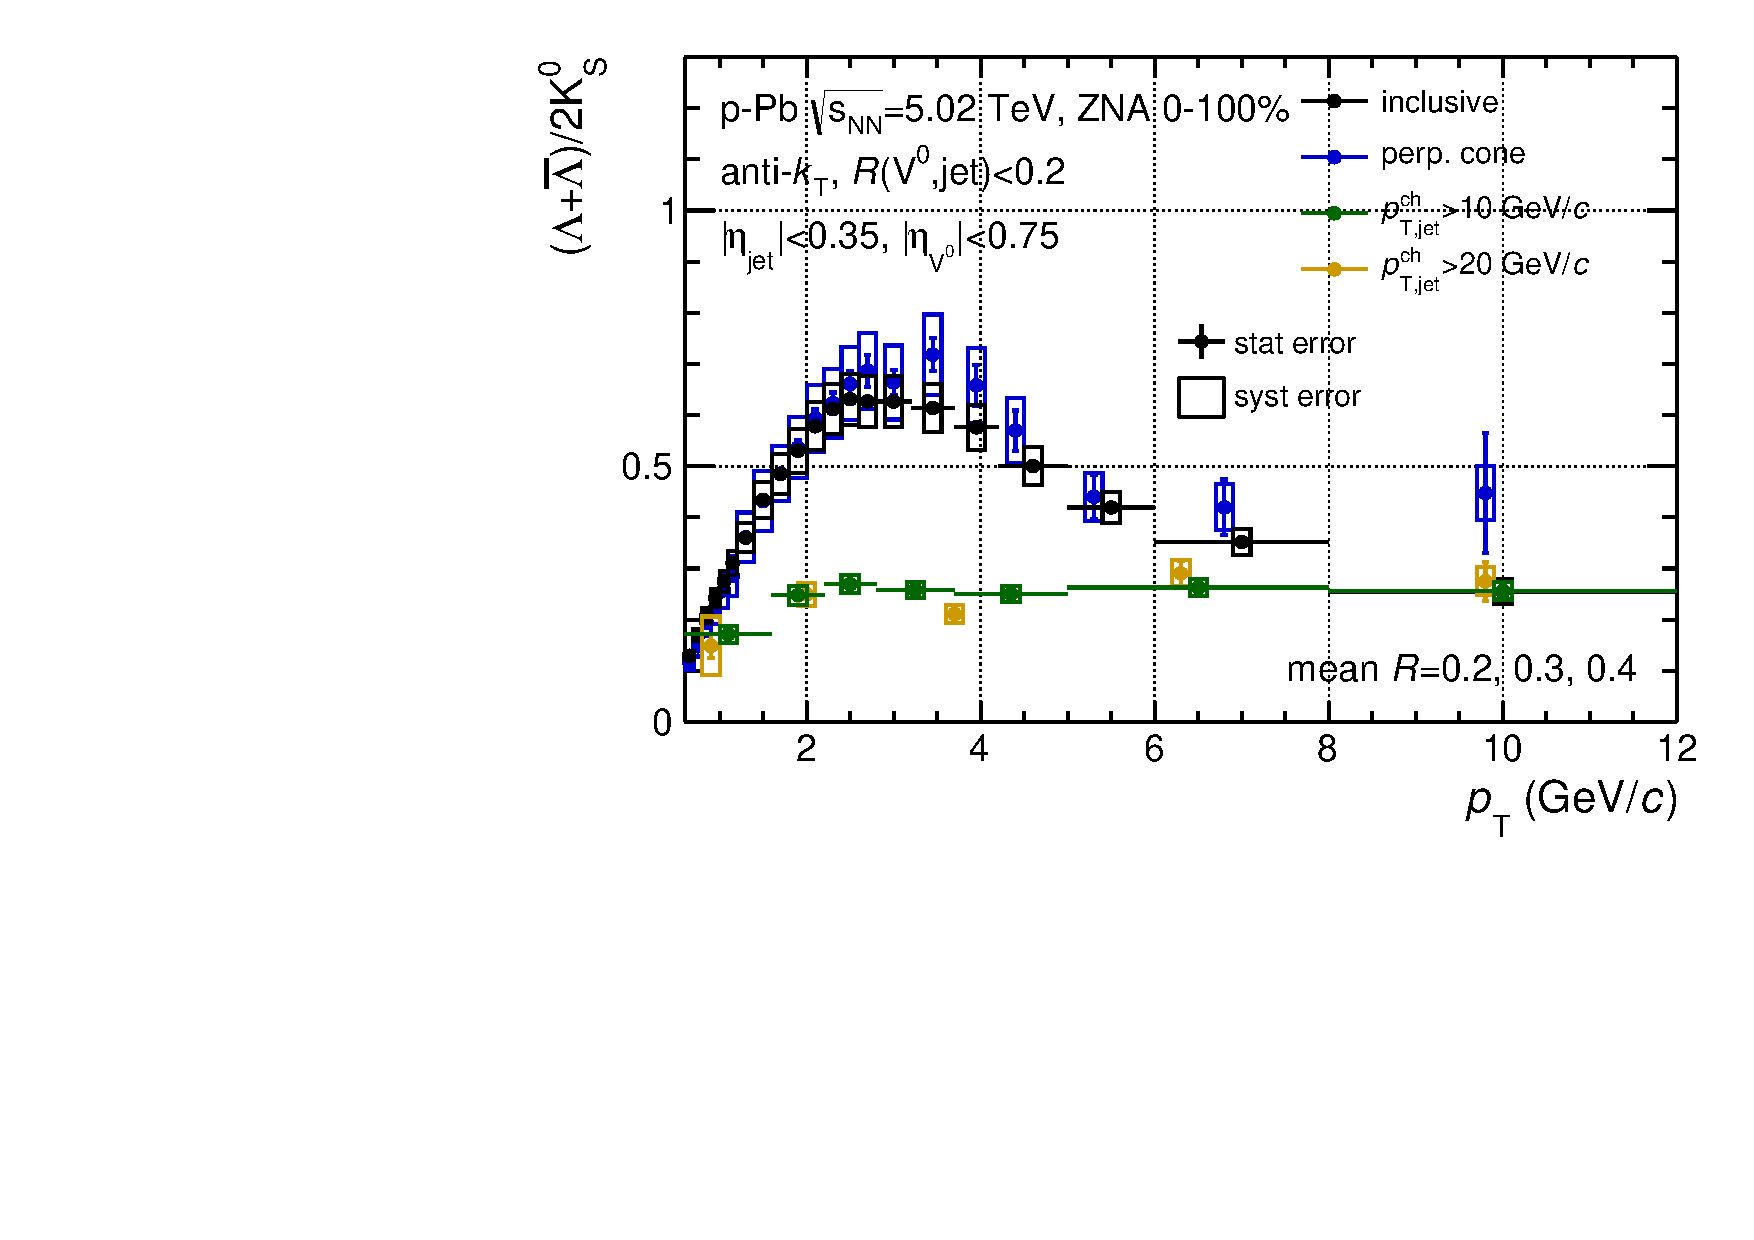
\includegraphics[width=.48\textwidth]{cL2K_Pt_PtJE_JC02_ZNA_000_100}
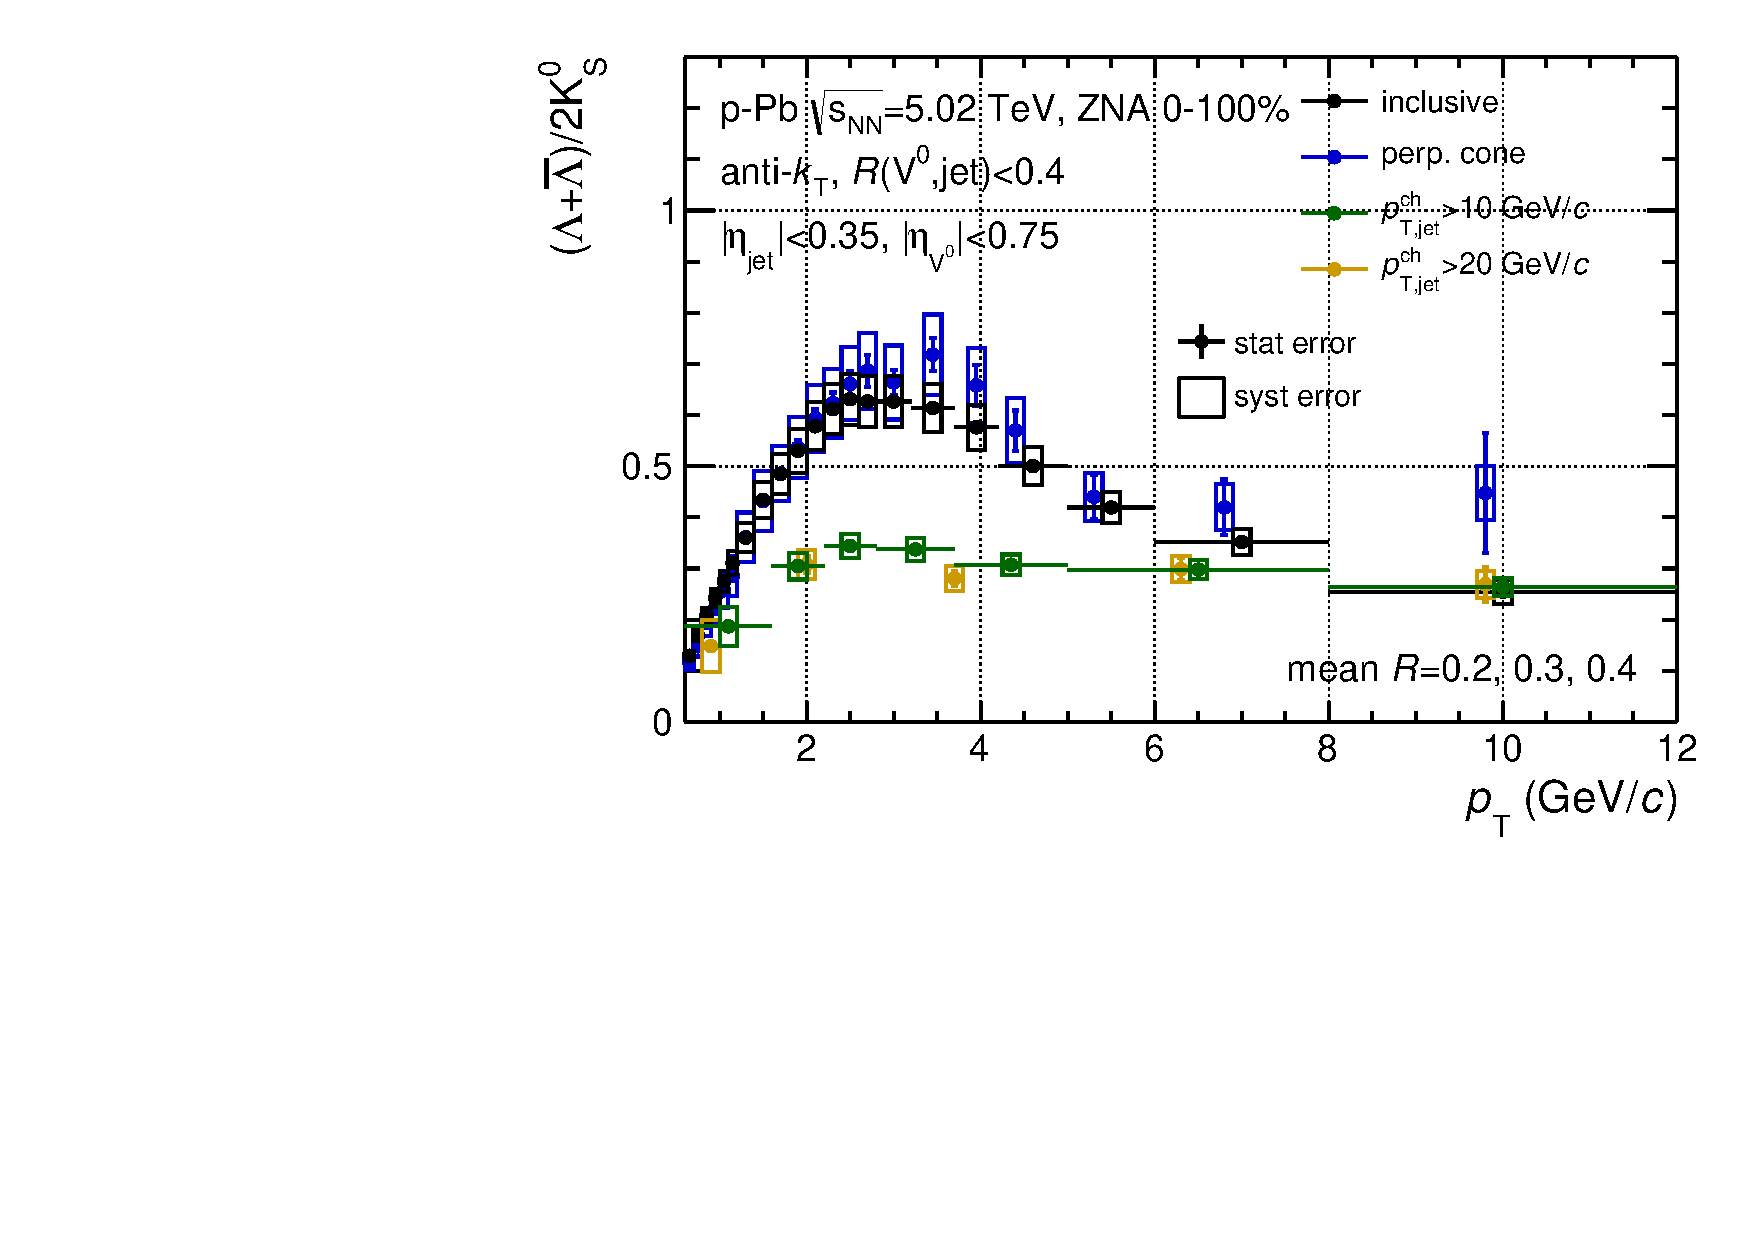
\includegraphics[width=.48\textwidth]{cL2K_Pt_PtJE_JC04_ZNA_000_100}
\caption{Systematic uncertainty of inclusive $\Vzero$s -- uncorrelated with statistics.}
\label{fig:c07LKration}
\end{center}
\end{figure}


\ask{all above for V0 and ZNA}

\subsection{\Vzero\ as a function of $R$}

\begin{figure}[t]
\begin{center}
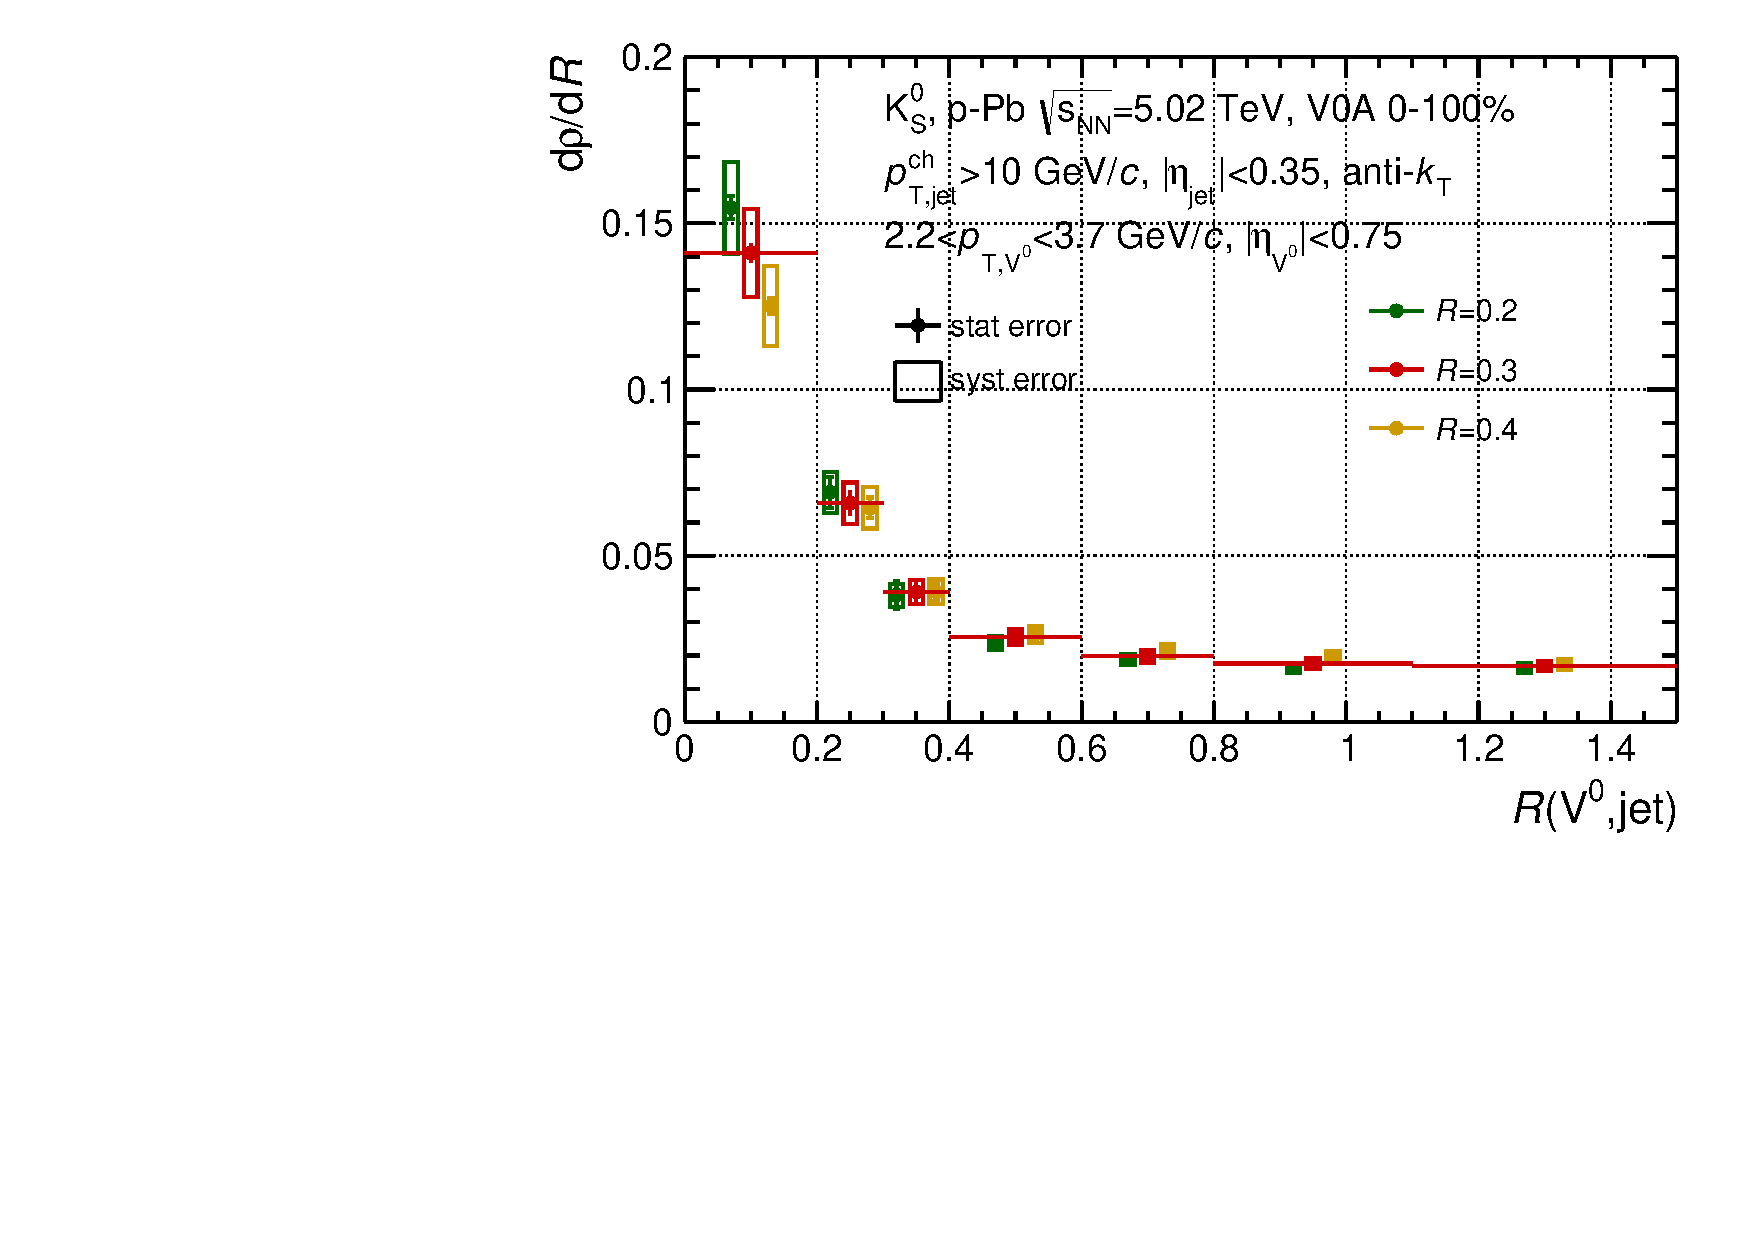
\includegraphics[width=.32\textwidth]{cKshort_VJ_Comp_V0A_000_100_PtJ10_PtV0_2d2_3d7}
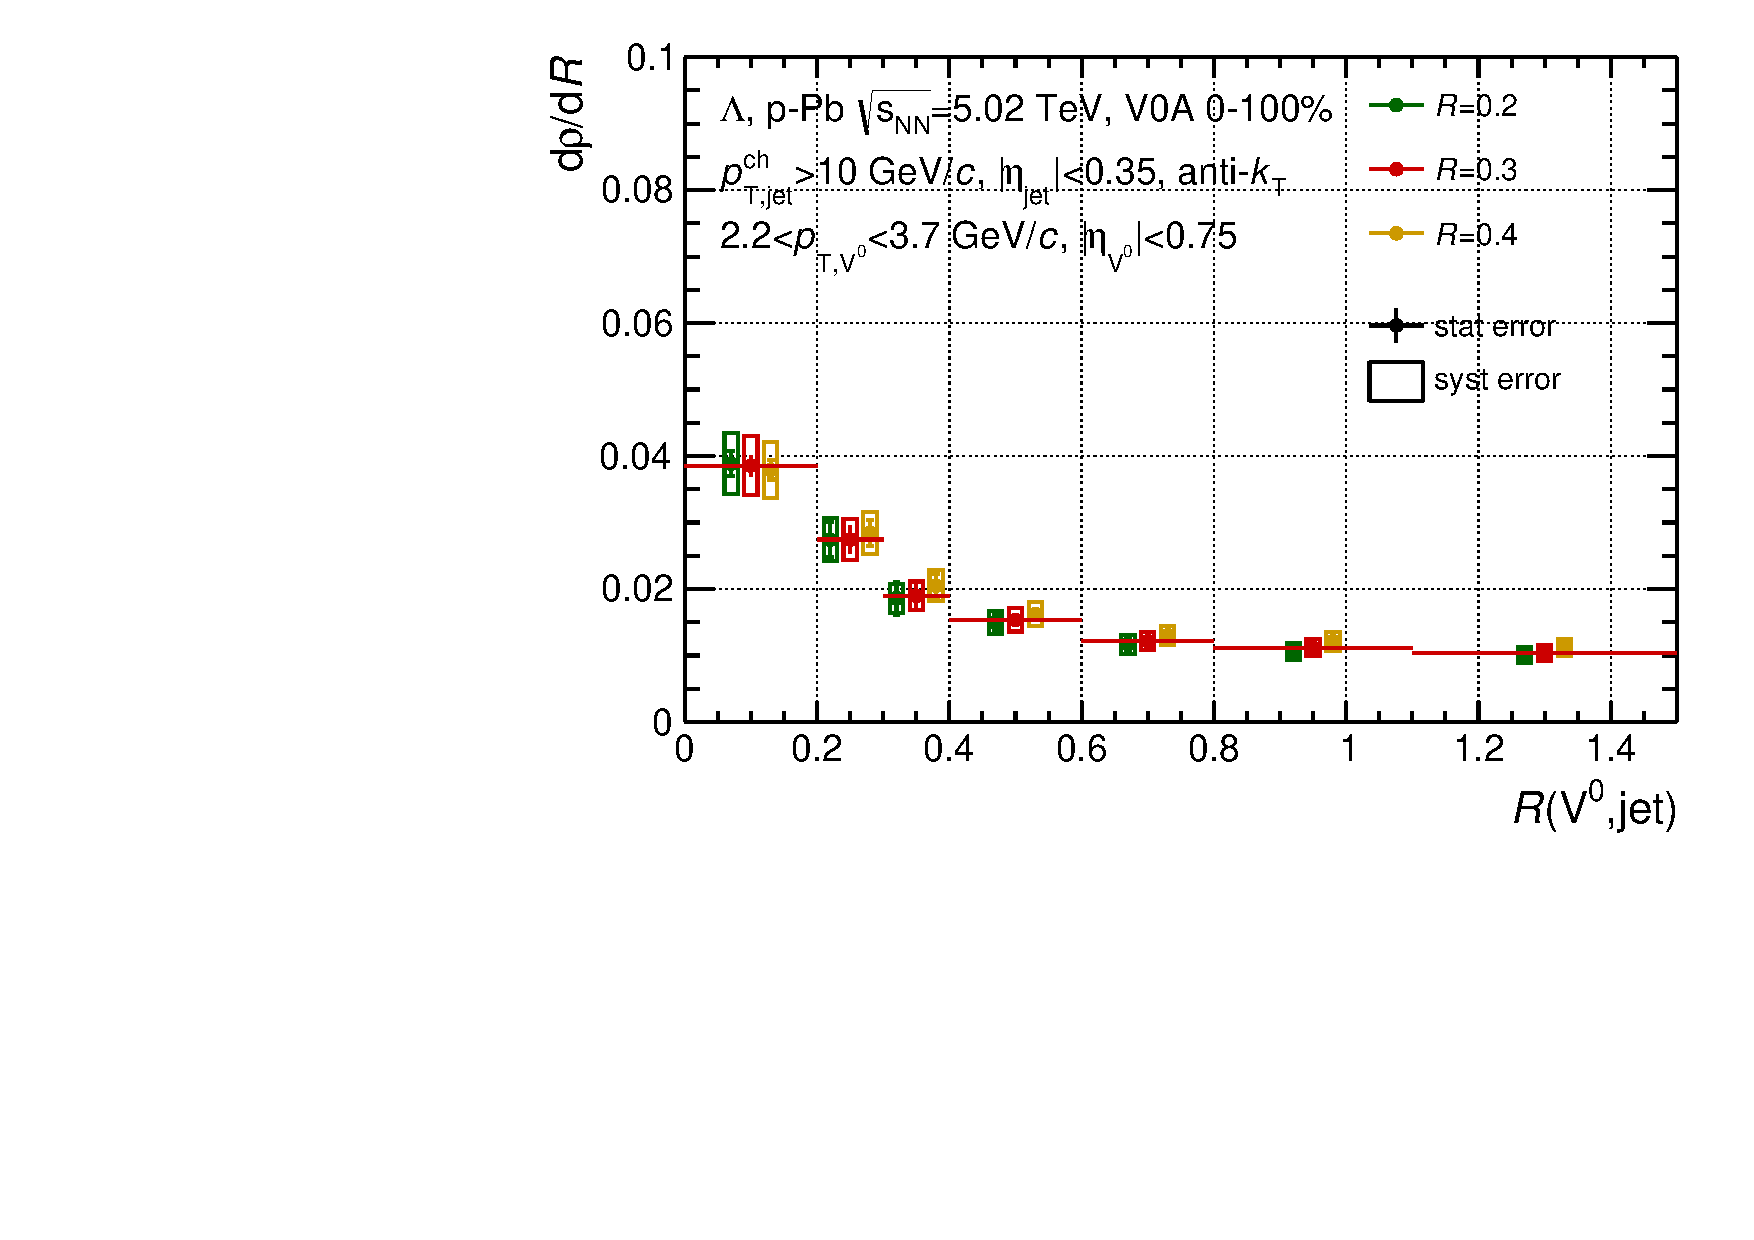
\includegraphics[width=.32\textwidth]{cLambda_VJ_Comp_V0A_000_100_PtJ10_PtV0_2d2_3d7}
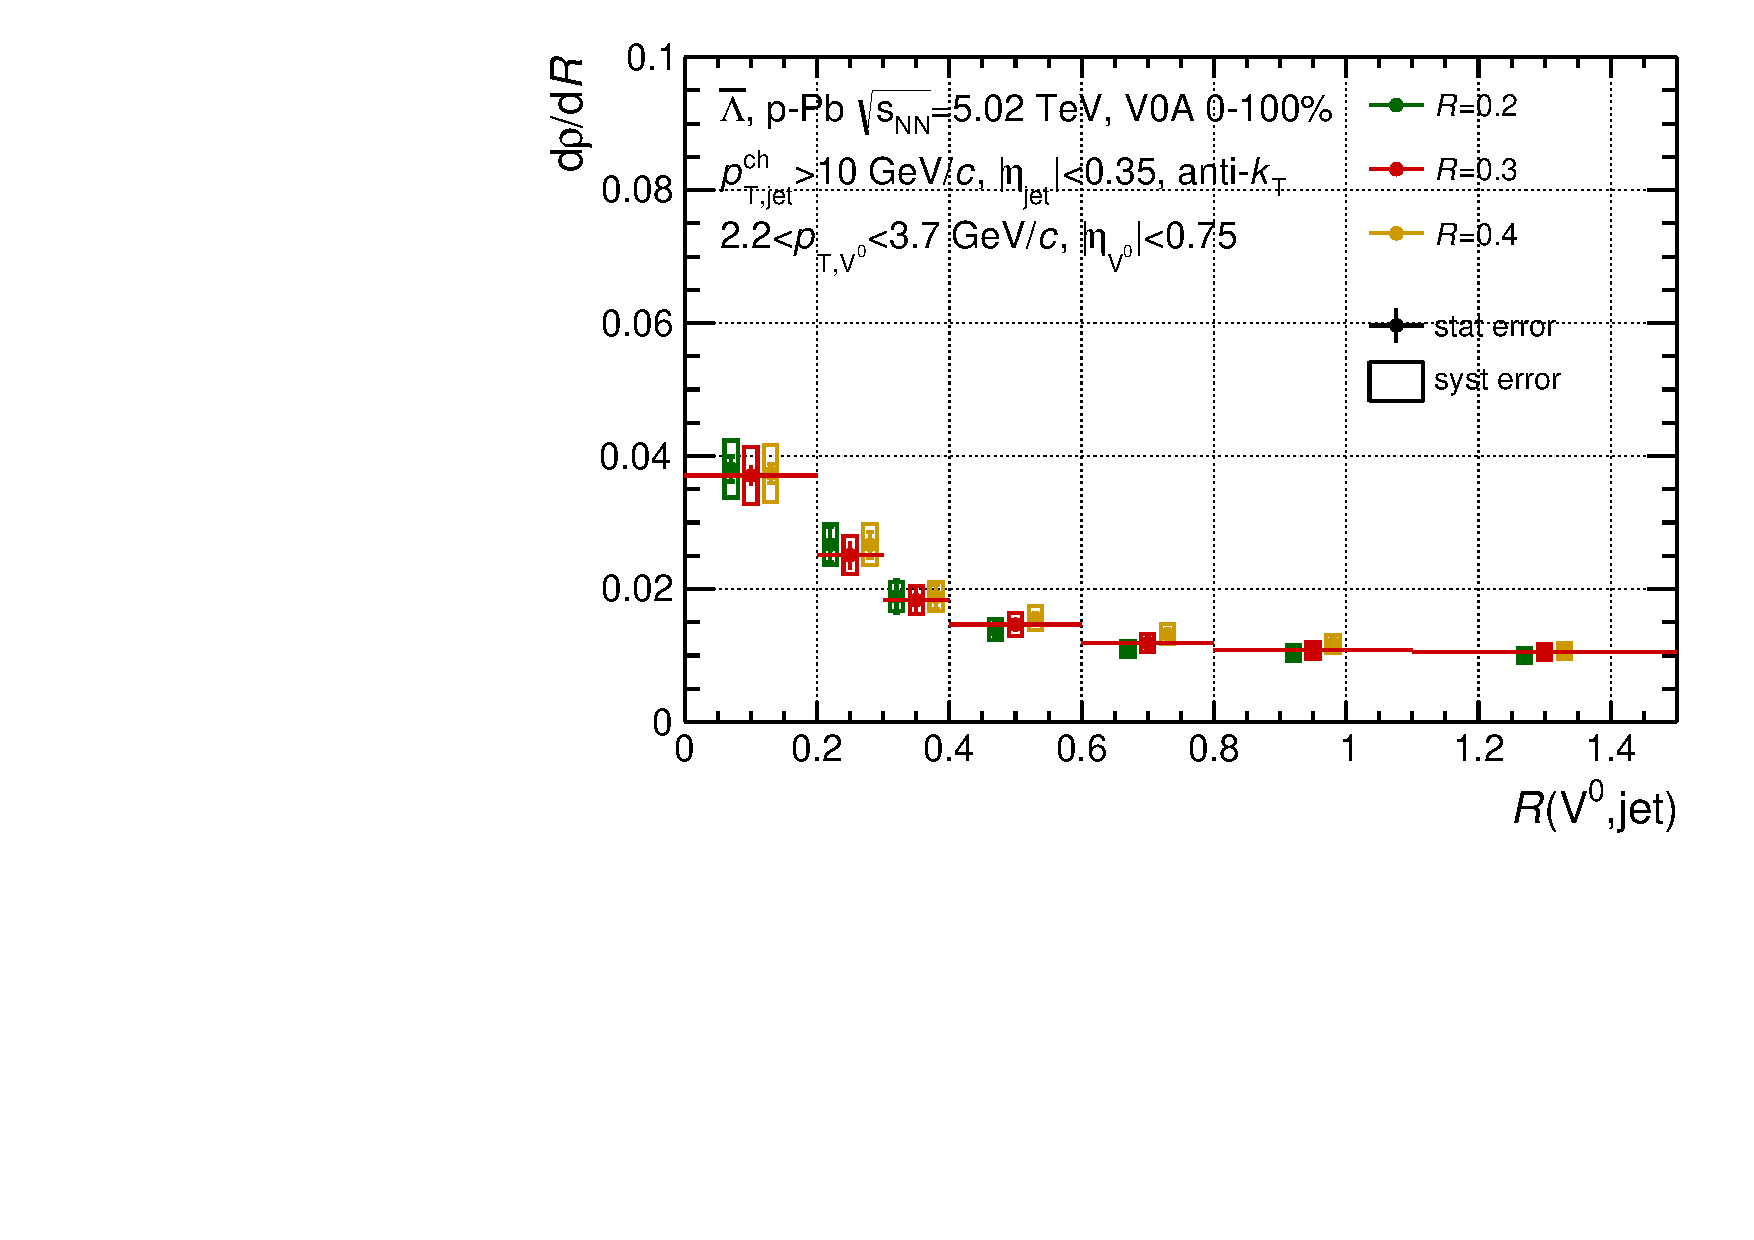
\includegraphics[width=.32\textwidth]{cAntiLa_VJ_Comp_V0A_000_100_PtJ10_PtV0_2d2_3d7}
\caption{$\Vzero$ density as a function of $R(\Vzero,{\rm jet})$.}
\label{fig:c07LKrhoR}
\end{center}
\end{figure}

\begin{figure}[t]
\begin{center}
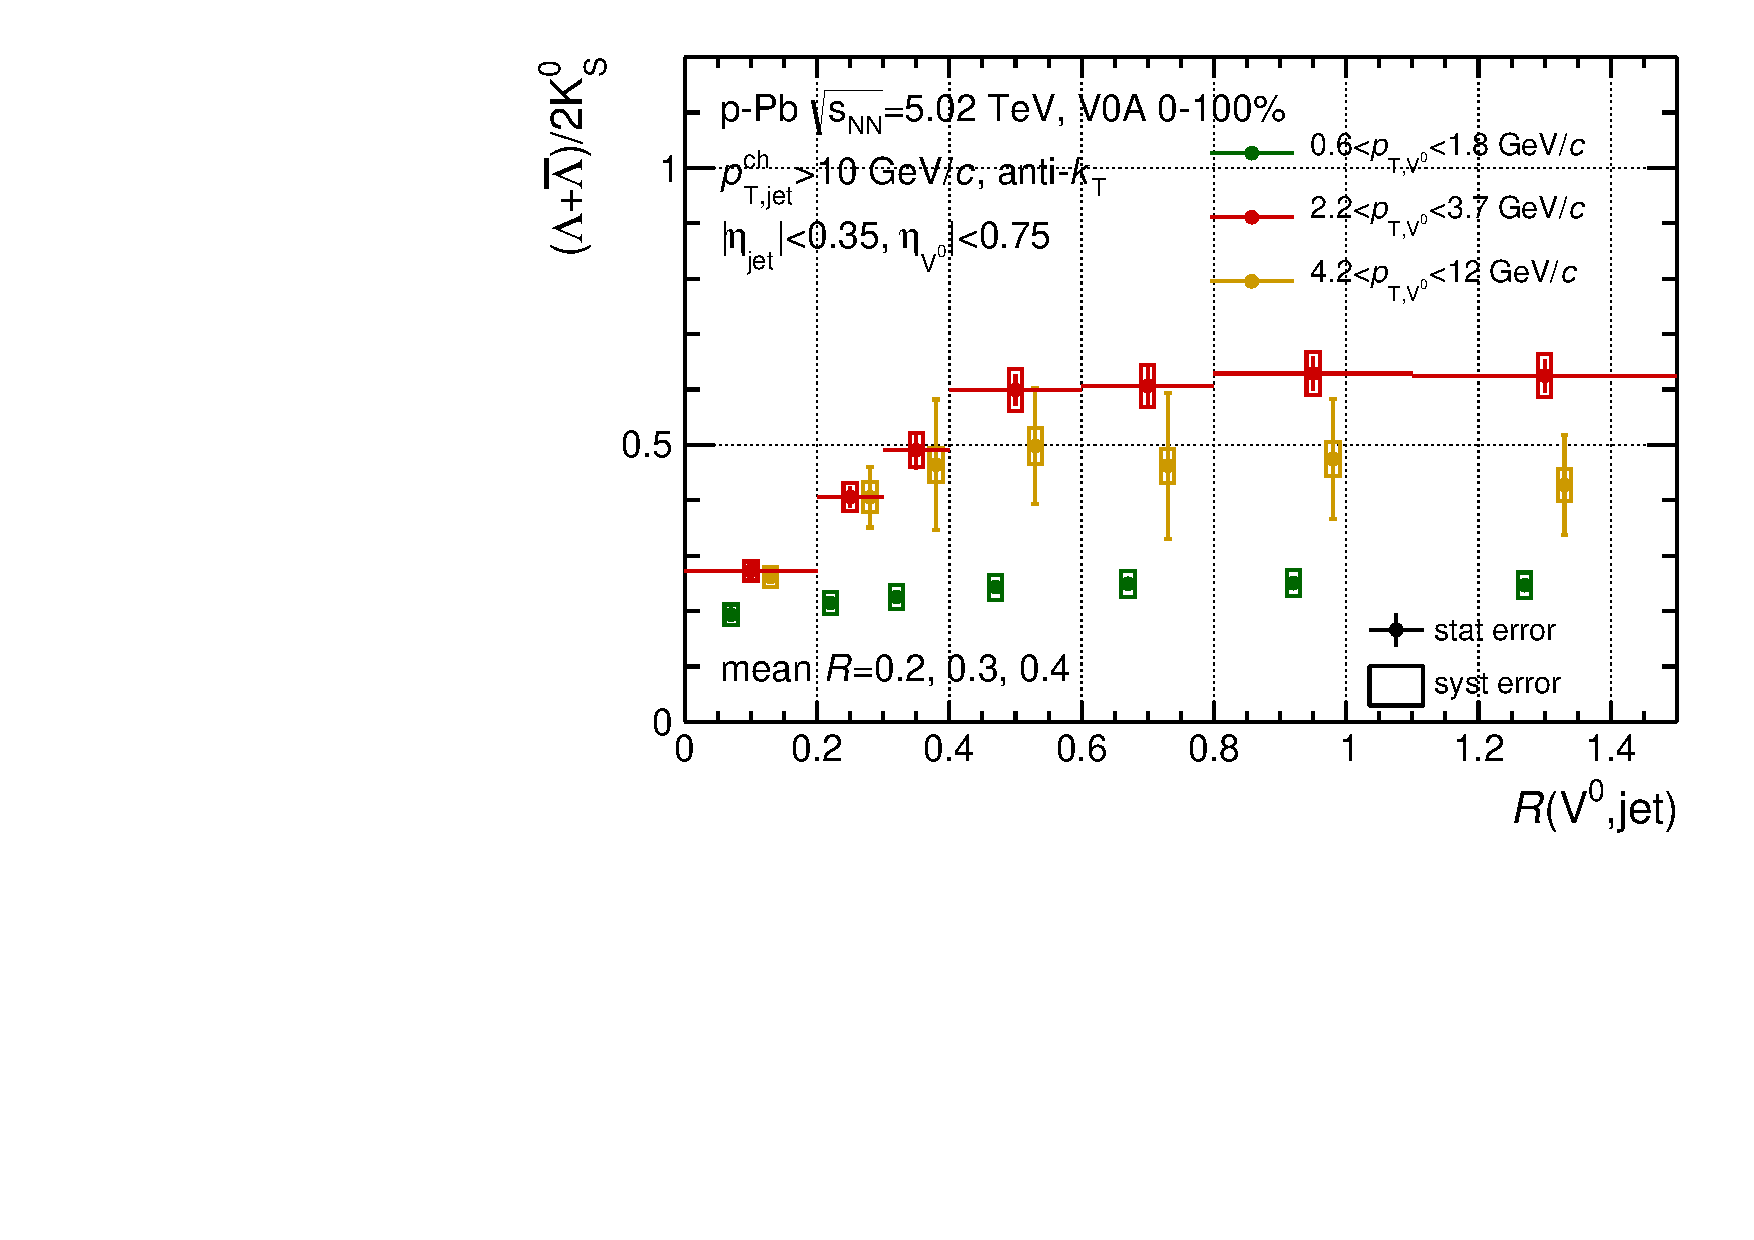
\includegraphics[width=.48\textwidth]{cRatioV_VJ_Mean_V0A_000_100_PtJ10}
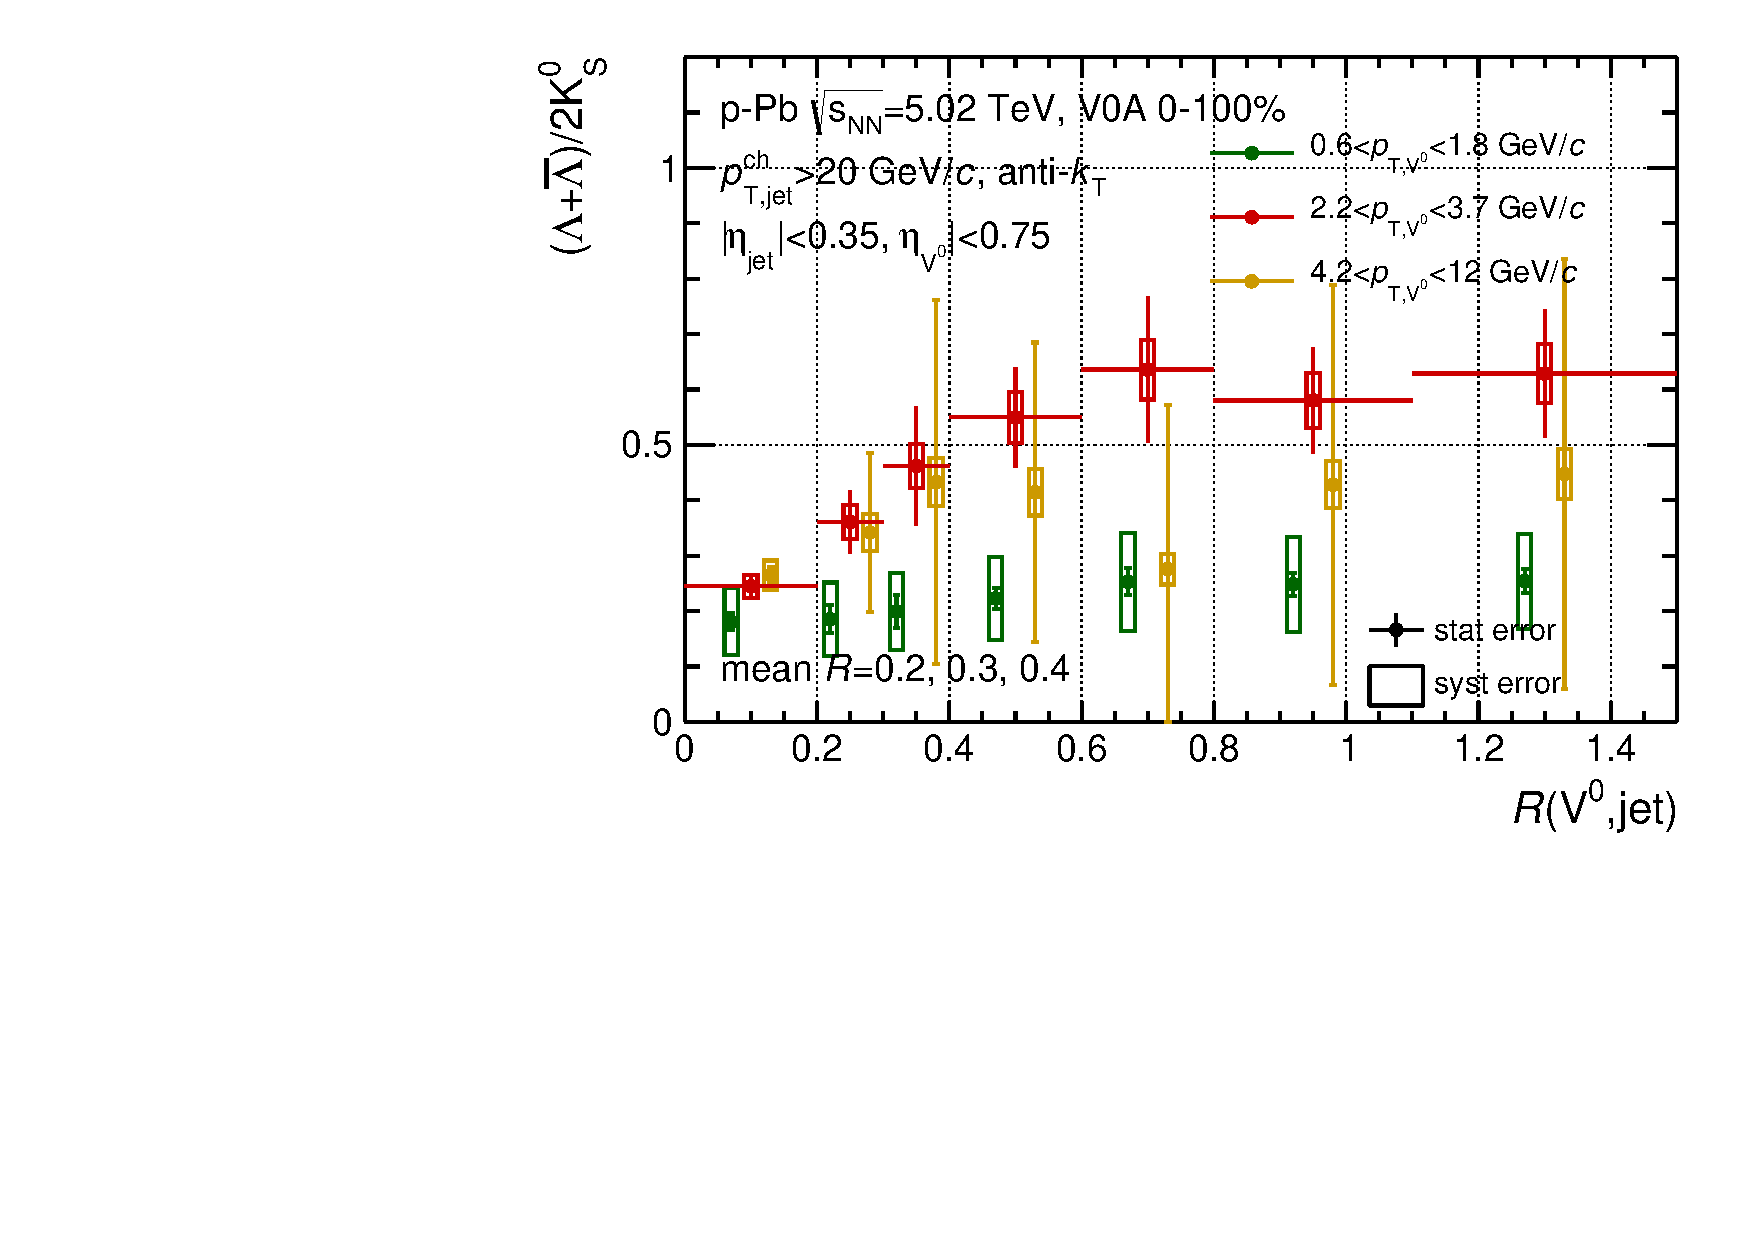
\includegraphics[width=.48\textwidth]{cRatioV_VJ_Mean_V0A_000_100_PtJ20}
\caption{L/K as a function of $R(\Vzero,{\rm jet})$.}
\label{fig:c07LKratioR}
\end{center}
\end{figure}

\subsection{mean \pt}

\ask{the mean \pt\ needs to be discussed; however, we may want to see the ratios}


\section{Summary}
\label{sec:con}

\begin{enumerate}
	\item spectra harder in jets
	\item L/K ratio: a) different than inclusive or OC/PC/NJ/inclusive - no peak; b) consistent with vacuum within uncertainties -> UE radial flow; jets do not flow
	\item mean \pt -> hint softening of jet fragments in most central collisions? - tension with 2.b
	\item constraint on the soft-hard parton recombination (?)
\end{enumerate}


%%%%%%%%%%%%%%%%%%%%%%%%%%%%%%%%%%%%%%%%%%%%%%%%%%%%%%%%%%%%%%%%%%%%%%%%%%%%%%%

\ifpreprint
  \iffull
    \newenvironment{acknowledgement}{\relax}{\relax}
    \begin{acknowledgement}
    \section*{Acknowledgements}
    The ALICE Collaboration would like to thank all its engineers and technicians
for their invaluable contributions to the construction of the experiment and
the CERN accelerator teams for the outstanding performance of the LHC complex.
%
The ALICE Collaboration gratefully acknowledges the resources and support
provided by all Grid centres and the Worldwide LHC Computing Grid (WLCG)
collaboration.
%
The ALICE Collaboration acknowledges the following funding agencies for
their support in building and running the ALICE detector:
%
State Committee of Science,  World Federation of Scientists (WFS)
and Swiss Fonds Kidagan, Armenia,
%
Conselho Nacional de Desenvolvimento Cient\'{\i}fico e Tecnol\'{o}gico (CNPq),
Financiadora de Estudos e Projetos (FINEP),
Funda\c{c}\~{a}o de Amparo \`{a} Pesquisa do Estado de S\~{a}o Paulo (FAPESP);
%
National Natural Science Foundation of China (NSFC),
the Chinese Ministry of Education (CMOE)
and the Ministry of Science and Technology of China (MSTC);
%
Ministry of Education and Youth of the Czech Republic;
%
Danish Natural Science Research Council,
the Carlsberg Foundation and the Danish National Research Foundation;
%
The European Research Council under the European Community's
Seventh Framework Programme;
%
Helsinki Institute of Physics and the Academy of Finland;
%
French CNRS-IN2P3,
the `Region Pays de Loire', `Region Alsace', `Region Auvergne' and CEA, France;
%
German Bundesministerium fur Bildung, Wissenschaft,
Forschung und Technologie (BMBF) and the Helmholtz Association;
%
General Secretariat for Research and Technology, Ministry of
Development, Greece;
%
Hungarian Orszagos Tudomanyos Kutatasi Alappgrammok (OTKA) and
National Office for Research and Technology (NKTH);
%
Department of Atomic Energy and Department of Science and Technology of the
Government of India;
%
Istituto Nazionale di Fisica Nucleare (INFN) and Centro Fermi -
Museo Storico della Fisica e Centro Studi e Ricerche "Enrico Fermi", Italy;
%
MEXT Grant-in-Aid for Specially Promoted Research, Ja\-pan;
%
Joint Institute for Nuclear Research, Dubna;
%
National Research Foundation of Korea (NRF);
%
Consejo Nacional de Cienca y Tecnologia (CONACYT),
Direccion General de Asuntos del Personal Academico(DGAPA),
M\'{e}xico, :Amerique Latine Formation academique –
European Commission(ALFA-EC) and the EPLANET Program (European
Particle Physics Latin American Network)
%
Stichting voor Fundamenteel Onderzoek der Materie (FOM) and
the Nederlandse Organisatie voor Wetenschappelijk Onderzoek (NWO), Netherlands;
%
Research Council of Norway (NFR);
%
Polish Ministry of Science and Higher Education;
%
National Science Centre, Poland;
%
Ministry of National Education/Institute for Atomic Physics and
Consiliul Naţional al Cercetării Ştiinţifice -
Executive Agency for Higher Education Research Development and
Innovation Funding (CNCS-UEFISCDI) - Romania;
%
Ministry of Education and Science of Russian Federation, Russian
Academy of Sciences, Russian Federal Agency of Atomic Energy,
Russian Federal Agency for Science and Innovations and The Russian
Foundation for Basic Research;
%
Ministry of Education of Slovakia;
%
Department of Science and Technology, South Africa;
%
Centro de Investigaciones Energeticas,
Medioambientales y Tecnologicas (CIEMAT),
E-Infrastructure shared between Europe and Latin America (EELA),
Ministerio de Econom\'{i}a y Competitividad (MINECO) of Spain,
Xunta de Galicia (Conseller\'{\i}a de Educaci\'{o}n),
Centro de Aplicaciones Tecnológicas y Desarrollo Nuclear (CEA\-DEN),
Cubaenerg\'{\i}a, Cuba, and IAEA (International Atomic Energy Agency);
%
Swedish Research Council (VR) and Knut $\&$ Alice Wallenberg
Foundation (KAW);
%
Ukraine Ministry of Education and Science;
%
United Kingdom Science and Technology Facilities Council (STFC);
%
The United States Department of Energy, the United States National
Science Foundation, the State of Texas, and the State of Ohio;
%
Ministry of Science, Education and
Sports of Croatia and  Unity through Knowledge Fund, Croatia.
%
Council of Scientific and Industrial Research (CSIR), New Delhi, India

    \end{acknowledgement}
%
    \ifbibtex
      \bibliographystyle{utphys}
      \bibliography{AliPubV0JetspPb}
    \else
      \input{refpreprint.tex}
    \fi
%
    \newpage
    \appendix
    \section{The ALICE Collaboration}
    \label{app:collab}
    \input{authors-preprint.tex}
  \else
    \ifbibtex
      \bibliographystyle{utphys}
      \bibliography{AliPubV0JetspPb}
    \else
      \ifpreprint
  \documentclass[ALICE,manyauthors,12pt]{cernphprep}
  \usepackage[comma,square,numbers,sort&compress]{natbib}
  \usepackage{booktabs}
\else %%% PUT PAPER STYLE BELOW %%%
  \ifplbpaper
  \documentclass[final,3p,12pt]{elsarticle}
  \biboptions{comma,square,numbers,sort&compress}
  \def\bibstname{utphys}
  \fi
%
  \ifapspaper
  \documentclass[10pt,aps,prl,superscriptaddress,altaffilletter,nobibnotes,nofootinbib]{revtex4-1}
  \newenvironment{frontmatter}{}{\maketitle}
  \def\bibstname{apsrev4-1}
  \fi
\fi
%%%%%%%%%%%%%%%%%%%%%%%%%%%%%%%%%%%%%%%%%%%%%%%%%%%%%%%%%%%%%%%%%%%%%%%%%%%%%%%

\ifdraft
  \usepackage{lineno}
  \linenumbers
  \setlength\linenumbersep{0.06in}
  \modulolinenumbers[5]
  \usepackage{fancyhdr}
  \pagestyle{fancyplain}
  \fancyhead{}
  \fancyhead[L,L]{\color{red}ALICE INTERNAL ONLY}
  \fancyhead[R,R]{\thepage}
  \fancyfoot{}
  \fancyfoot[L,L]{\color{red}DRAFT \dvers\ \revision $\color{white}:$\$}
  \fancyfoot[R,R]{\color{red} \today $\color{white}:$\$}
  \renewcommand{\headrulewidth}{0pt} % remove lines as well
  \renewcommand{\footrulewidth}{0pt}
  \newcommand{\ask}[1]{\textcolor{magenta}{#1}}
\else
  \newcommand{\ask}[1]{}
\fi
%%%%%%%%%%%%%%%%%%%%%%%%%%%%%%%%%%%%%%%%%%%%%%%%%%%%%%%%%%%%%%%%%%%%%%%%%%%%%%%

\iflatexdiff
  \RequirePackage{color}
  \definecolor{RED}{rgb}{1,0,0}
  \definecolor{BLUE}{rgb}{0,0,1}
  \providecommand{\DIFadd}[1]{{\protect\color{blue}\uwave{#1}}}
  \providecommand{\DIFdel}[1]{{\protect\color{red}\sout{#1}}}
  \providecommand{\DIFaddbegin}{}
  \providecommand{\DIFaddend}{}
  \providecommand{\DIFdelbegin}{}
  \providecommand{\DIFdelend}{}
  \providecommand{\DIFaddFL}[1]{\DIFadd{#1}}
  \providecommand{\DIFdelFL}[1]{\DIFdel{#1}}
  \providecommand{\DIFaddbeginFL}{}
  \providecommand{\DIFaddendFL}{}
  \providecommand{\DIFdelbeginFL}{}
  \providecommand{\DIFdelendFL}{}
\fi
%==========================================================%

\usepackage{float}
\usepackage{rotating}

\usepackage{graphicx}
\usepackage{graphics}
\usepackage{epstopdf}
\usepackage{epsfig}
\usepackage{grffile}

\usepackage{dcolumn}
\usepackage{multirow}
\usepackage{array}

\usepackage{bm}
\usepackage{amsmath}
\usepackage{amssymb}
\usepackage{amsfonts}

\usepackage{units}
\usepackage{hyperref}

\usepackage{color}
%\usepackage[usenames]{color}

\usepackage{textcomp}
\usepackage[normalem]{ulem}
\usepackage[utf8]{inputenc}
\usepackage[T1]{fontenc}

%usepackage{changes}
%usepackage{lipsum}
%definechangesauthor[name={Xiaoming Zhang}, color=orange]{xz}
%definechangesauthor[name={MP}, color=orange]{mp}
%setremarkmarkup{(#2)}
%%%%%%%%%%%%%%%%%%%%%%%%%%%%%%%%%%%%%%%%%%%%%%%%%%%%%%%%%%%%%%%%%%%%%%%%%%%%%%%

\graphicspath{{figures/}
              {figures/c00Logos/}
              {figures/c23V0Reco/}
              {figures/c24Syst/}
              {figures/c03Results/}}
%%%%%%%%%%%%%%%%%%%%%%%%%%%%%%%%%%%%%%%%%%%%%%%%%%%%%%%%%%%%%%%%%%%%%%%%%%%%%%%

\newcolumntype{P}[1]{>{\centering\arraybackslash}p{#1}}
\newcolumntype{M}[1]{>{\centering\arraybackslash}m{#1}}
%%%%%%%%%%%%%%%%%%%%%%%%%%%%%%%%%%%%%%%%%%%%%%%%%%%%%%%%%%%%%%%%%%%%%%%%%%%%%%%

\newcommand{\murm}{%
  \ifmmode
    \mathchoice
        {\hbox{\normalsize\textmu}}
        {\hbox{\normalsize\textmu}}
        {\hbox{\scriptsize\textmu}}
        {\hbox{\tiny\textmu}}%
  \else
    \textmu
  \fi
}
%%%%%%%%%%%%%%%%%%%%%%%%%%%%%%%%%%%%%%%%%%%%%%%%%%%%%%%%%%%%%%%%%%%%%%%%%%%%%%%

\newcommand{\pip}{\ensuremath{\pi^{+}}}
\newcommand{\pim}{\ensuremath{\pi^{-}}}
\newcommand{\kap}{\ensuremath{{\rm K}^{+}}}
\newcommand{\kam}{\ensuremath{{\rm K}^{-}}}
\newcommand{\pbar}{\ensuremath{\rm\overline{p}}}
\newcommand{\degree}{\ensuremath{^{\rm o}}}
\newcommand{\s}{\ensuremath{\sqrt{s}}}
\newcommand{\pt}{\ensuremath{p_{\rm t}}}
\newcommand{\dedx}{\ensuremath{{\rm d}E/{\rm d}x}}
\newcommand{\dndy}{\ensuremath{{\rm d}N/{\rm d}y}}
\newcommand{\dndydpt}{\ensuremath{{\rm d}^{2}N/{\rm d}y{\rm d}p_{\rm t}}}
\newcommand{\pp}{pp}

\newcommand{\jpsi}{\ensuremath{{\rm J/}\psi}}
\newcommand{\psip}{\ensuremath{\psi^{\prime}}}
\newcommand{\jpsiDY}{\ensuremath{{\rm J/}\psi{\rm ,/,DY}}}
\newcommand{\dd}{\ensuremath{{\rm d}}}
\newcommand{\chic}{\ensuremath{\chi_{\rm c}}}
\newcommand{\ezdc}{\ensuremath {E_{\rm ZDC}}}
\newcommand{\red}{\textcolor{red}}
\newcommand{\blue}{\textcolor{blue}}

\newcommand{\slfrac}[2]{\left.#1\right/#2}
%%%%%%%%%%%%%%%%%%%%%%%%%%%%%%%%%%%%%%%%%%%%%%%%%%%%%%%%%%%%%%%%%%%%%%%%%%%%%%%

\newcommand{\abs}[1]{\ensuremath{\left|#1\right|}}
\newcommand{\avg}[1]{\ensuremath{\left\langle #1\right\rangle}}

\newcommand{\pT}[1][T]{\ifthenelse{\equal{#1}{T}}
                                  {\ensuremath{p_{\rm #1}}}
                                  {\ensuremath{p_{\rm T,#1}}}}

\newcommand{\dndydpT}{\ensuremath{{\rm d}^{2}N/{\rm d}y{\rm d}p_{\rm T}}}
\newcommand{\dtod}[2]{\ensuremath{{\rm d}#1/{\rm d}#2}}
\newcommand{\dtodd}[3]{\ensuremath{{\rm d}^{2}#1/{\rm d}#2{\rm d}#3}}
%%%%%%%%%%%%%%%%%%%%%%%%%%%%%%%%%%%%%%%%%%%%%%%%%%%%%%%%%%%%%%%%%%%%%%%%%%%%%%%

\newcommand{\GeVc} {\ensuremath{{\rm GeV/}c}}
\newcommand{\GeVcc}{\ensuremath{{\rm GeV/}c^{2}}}

\newcommand{\MeVc} {\ensuremath{{\rm MeV/}c}}
\newcommand{\MeVcc}{\ensuremath{{\rm MeV/}c^{2}}}

\newcommand{\sNN}{\ensuremath{\sqrt{s_{\rm NN}}}}
\newcommand{\hlab}{\ensuremath{\eta_{\rm lab}}}
\newcommand{\yCMS}{\ensuremath{y_{\rm CMS}}}
\newcommand{\yNN}{\ensuremath{y_{\rm NN}}}

\newcommand{\kT}{\ensuremath{k_{\rm T}}}
\newcommand{\Ajet}{\ensuremath{A_{\rm jet}}}
\newcommand{\RAA}{\ensuremath{R_{\rm AA}}}

\newcommand{\Vzero}{\ensuremath{{\rm V}^{0}}}
\newcommand{\Kshort}{\ensuremath{{\rm K}_{\rm S}^{0}}}
\newcommand{\AntiLa}{\ensuremath{\overline{\Lambda}}}

\newcommand{\qhat}{\ensuremath{\hat{q}}}
\newcommand{\cent}[2]{$#1$--$#2\%$}
%%%%%%%%%%%%%%%%%%%%%%%%%%%%%%%%%%%%%%%%%%%%%%%%%%%%%%%%%%%%%%%%%%%%%%%%%%%%%%%

    \fi
  \fi
\else
  \iffull
    \vspace{0.5cm}
    The ALICE Collaboration would like to thank all its engineers and technicians
for their invaluable contributions to the construction of the experiment and
the CERN accelerator teams for the outstanding performance of the LHC complex.
%
The ALICE Collaboration gratefully acknowledges the resources and support
provided by all Grid centres and the Worldwide LHC Computing Grid (WLCG)
collaboration.
%
The ALICE Collaboration acknowledges the following funding agencies for
their support in building and running the ALICE detector:
%
State Committee of Science,  World Federation of Scientists (WFS)
and Swiss Fonds Kidagan, Armenia,
%
Conselho Nacional de Desenvolvimento Cient\'{\i}fico e Tecnol\'{o}gico (CNPq),
Financiadora de Estudos e Projetos (FINEP),
Funda\c{c}\~{a}o de Amparo \`{a} Pesquisa do Estado de S\~{a}o Paulo (FAPESP);
%
National Natural Science Foundation of China (NSFC),
the Chinese Ministry of Education (CMOE)
and the Ministry of Science and Technology of China (MSTC);
%
Ministry of Education and Youth of the Czech Republic;
%
Danish Natural Science Research Council,
the Carlsberg Foundation and the Danish National Research Foundation;
%
The European Research Council under the European Community's
Seventh Framework Programme;
%
Helsinki Institute of Physics and the Academy of Finland;
%
French CNRS-IN2P3,
the `Region Pays de Loire', `Region Alsace', `Region Auvergne' and CEA, France;
%
German Bundesministerium fur Bildung, Wissenschaft,
Forschung und Technologie (BMBF) and the Helmholtz Association;
%
General Secretariat for Research and Technology, Ministry of
Development, Greece;
%
Hungarian Orszagos Tudomanyos Kutatasi Alappgrammok (OTKA) and
National Office for Research and Technology (NKTH);
%
Department of Atomic Energy and Department of Science and Technology of the
Government of India;
%
Istituto Nazionale di Fisica Nucleare (INFN) and Centro Fermi -
Museo Storico della Fisica e Centro Studi e Ricerche "Enrico Fermi", Italy;
%
MEXT Grant-in-Aid for Specially Promoted Research, Ja\-pan;
%
Joint Institute for Nuclear Research, Dubna;
%
National Research Foundation of Korea (NRF);
%
Consejo Nacional de Cienca y Tecnologia (CONACYT),
Direccion General de Asuntos del Personal Academico(DGAPA),
M\'{e}xico, :Amerique Latine Formation academique –
European Commission(ALFA-EC) and the EPLANET Program (European
Particle Physics Latin American Network)
%
Stichting voor Fundamenteel Onderzoek der Materie (FOM) and
the Nederlandse Organisatie voor Wetenschappelijk Onderzoek (NWO), Netherlands;
%
Research Council of Norway (NFR);
%
Polish Ministry of Science and Higher Education;
%
National Science Centre, Poland;
%
Ministry of National Education/Institute for Atomic Physics and
Consiliul Naţional al Cercetării Ştiinţifice -
Executive Agency for Higher Education Research Development and
Innovation Funding (CNCS-UEFISCDI) - Romania;
%
Ministry of Education and Science of Russian Federation, Russian
Academy of Sciences, Russian Federal Agency of Atomic Energy,
Russian Federal Agency for Science and Innovations and The Russian
Foundation for Basic Research;
%
Ministry of Education of Slovakia;
%
Department of Science and Technology, South Africa;
%
Centro de Investigaciones Energeticas,
Medioambientales y Tecnologicas (CIEMAT),
E-Infrastructure shared between Europe and Latin America (EELA),
Ministerio de Econom\'{i}a y Competitividad (MINECO) of Spain,
Xunta de Galicia (Conseller\'{\i}a de Educaci\'{o}n),
Centro de Aplicaciones Tecnológicas y Desarrollo Nuclear (CEA\-DEN),
Cubaenerg\'{\i}a, Cuba, and IAEA (International Atomic Energy Agency);
%
Swedish Research Council (VR) and Knut $\&$ Alice Wallenberg
Foundation (KAW);
%
Ukraine Ministry of Education and Science;
%
United Kingdom Science and Technology Facilities Council (STFC);
%
The United States Department of Energy, the United States National
Science Foundation, the State of Texas, and the State of Ohio;
%
Ministry of Science, Education and
Sports of Croatia and  Unity through Knowledge Fund, Croatia.
%
Council of Scientific and Industrial Research (CSIR), New Delhi, India

    \ifpreprint
  \documentclass[ALICE,manyauthors,12pt]{cernphprep}
  \usepackage[comma,square,numbers,sort&compress]{natbib}
  \usepackage{booktabs}
\else %%% PUT PAPER STYLE BELOW %%%
  \ifplbpaper
  \documentclass[final,3p,12pt]{elsarticle}
  \biboptions{comma,square,numbers,sort&compress}
  \def\bibstname{utphys}
  \fi
%
  \ifapspaper
  \documentclass[10pt,aps,prl,superscriptaddress,altaffilletter,nobibnotes,nofootinbib]{revtex4-1}
  \newenvironment{frontmatter}{}{\maketitle}
  \def\bibstname{apsrev4-1}
  \fi
\fi
%%%%%%%%%%%%%%%%%%%%%%%%%%%%%%%%%%%%%%%%%%%%%%%%%%%%%%%%%%%%%%%%%%%%%%%%%%%%%%%

\ifdraft
  \usepackage{lineno}
  \linenumbers
  \setlength\linenumbersep{0.06in}
  \modulolinenumbers[5]
  \usepackage{fancyhdr}
  \pagestyle{fancyplain}
  \fancyhead{}
  \fancyhead[L,L]{\color{red}ALICE INTERNAL ONLY}
  \fancyhead[R,R]{\thepage}
  \fancyfoot{}
  \fancyfoot[L,L]{\color{red}DRAFT \dvers\ \revision $\color{white}:$\$}
  \fancyfoot[R,R]{\color{red} \today $\color{white}:$\$}
  \renewcommand{\headrulewidth}{0pt} % remove lines as well
  \renewcommand{\footrulewidth}{0pt}
  \newcommand{\ask}[1]{\textcolor{magenta}{#1}}
\else
  \newcommand{\ask}[1]{}
\fi
%%%%%%%%%%%%%%%%%%%%%%%%%%%%%%%%%%%%%%%%%%%%%%%%%%%%%%%%%%%%%%%%%%%%%%%%%%%%%%%

\iflatexdiff
  \RequirePackage{color}
  \definecolor{RED}{rgb}{1,0,0}
  \definecolor{BLUE}{rgb}{0,0,1}
  \providecommand{\DIFadd}[1]{{\protect\color{blue}\uwave{#1}}}
  \providecommand{\DIFdel}[1]{{\protect\color{red}\sout{#1}}}
  \providecommand{\DIFaddbegin}{}
  \providecommand{\DIFaddend}{}
  \providecommand{\DIFdelbegin}{}
  \providecommand{\DIFdelend}{}
  \providecommand{\DIFaddFL}[1]{\DIFadd{#1}}
  \providecommand{\DIFdelFL}[1]{\DIFdel{#1}}
  \providecommand{\DIFaddbeginFL}{}
  \providecommand{\DIFaddendFL}{}
  \providecommand{\DIFdelbeginFL}{}
  \providecommand{\DIFdelendFL}{}
\fi
%==========================================================%

\usepackage{float}
\usepackage{rotating}

\usepackage{graphicx}
\usepackage{graphics}
\usepackage{epstopdf}
\usepackage{epsfig}
\usepackage{grffile}

\usepackage{dcolumn}
\usepackage{multirow}
\usepackage{array}

\usepackage{bm}
\usepackage{amsmath}
\usepackage{amssymb}
\usepackage{amsfonts}

\usepackage{units}
\usepackage{hyperref}

\usepackage{color}
%\usepackage[usenames]{color}

\usepackage{textcomp}
\usepackage[normalem]{ulem}
\usepackage[utf8]{inputenc}
\usepackage[T1]{fontenc}

%usepackage{changes}
%usepackage{lipsum}
%definechangesauthor[name={Xiaoming Zhang}, color=orange]{xz}
%definechangesauthor[name={MP}, color=orange]{mp}
%setremarkmarkup{(#2)}
%%%%%%%%%%%%%%%%%%%%%%%%%%%%%%%%%%%%%%%%%%%%%%%%%%%%%%%%%%%%%%%%%%%%%%%%%%%%%%%

\graphicspath{{figures/}
              {figures/c00Logos/}
              {figures/c23V0Reco/}
              {figures/c24Syst/}
              {figures/c03Results/}}
%%%%%%%%%%%%%%%%%%%%%%%%%%%%%%%%%%%%%%%%%%%%%%%%%%%%%%%%%%%%%%%%%%%%%%%%%%%%%%%

\newcolumntype{P}[1]{>{\centering\arraybackslash}p{#1}}
\newcolumntype{M}[1]{>{\centering\arraybackslash}m{#1}}
%%%%%%%%%%%%%%%%%%%%%%%%%%%%%%%%%%%%%%%%%%%%%%%%%%%%%%%%%%%%%%%%%%%%%%%%%%%%%%%

\newcommand{\murm}{%
  \ifmmode
    \mathchoice
        {\hbox{\normalsize\textmu}}
        {\hbox{\normalsize\textmu}}
        {\hbox{\scriptsize\textmu}}
        {\hbox{\tiny\textmu}}%
  \else
    \textmu
  \fi
}
%%%%%%%%%%%%%%%%%%%%%%%%%%%%%%%%%%%%%%%%%%%%%%%%%%%%%%%%%%%%%%%%%%%%%%%%%%%%%%%

\newcommand{\pip}{\ensuremath{\pi^{+}}}
\newcommand{\pim}{\ensuremath{\pi^{-}}}
\newcommand{\kap}{\ensuremath{{\rm K}^{+}}}
\newcommand{\kam}{\ensuremath{{\rm K}^{-}}}
\newcommand{\pbar}{\ensuremath{\rm\overline{p}}}
\newcommand{\degree}{\ensuremath{^{\rm o}}}
\newcommand{\s}{\ensuremath{\sqrt{s}}}
\newcommand{\pt}{\ensuremath{p_{\rm t}}}
\newcommand{\dedx}{\ensuremath{{\rm d}E/{\rm d}x}}
\newcommand{\dndy}{\ensuremath{{\rm d}N/{\rm d}y}}
\newcommand{\dndydpt}{\ensuremath{{\rm d}^{2}N/{\rm d}y{\rm d}p_{\rm t}}}
\newcommand{\pp}{pp}

\newcommand{\jpsi}{\ensuremath{{\rm J/}\psi}}
\newcommand{\psip}{\ensuremath{\psi^{\prime}}}
\newcommand{\jpsiDY}{\ensuremath{{\rm J/}\psi{\rm ,/,DY}}}
\newcommand{\dd}{\ensuremath{{\rm d}}}
\newcommand{\chic}{\ensuremath{\chi_{\rm c}}}
\newcommand{\ezdc}{\ensuremath {E_{\rm ZDC}}}
\newcommand{\red}{\textcolor{red}}
\newcommand{\blue}{\textcolor{blue}}

\newcommand{\slfrac}[2]{\left.#1\right/#2}
%%%%%%%%%%%%%%%%%%%%%%%%%%%%%%%%%%%%%%%%%%%%%%%%%%%%%%%%%%%%%%%%%%%%%%%%%%%%%%%

\newcommand{\abs}[1]{\ensuremath{\left|#1\right|}}
\newcommand{\avg}[1]{\ensuremath{\left\langle #1\right\rangle}}

\newcommand{\pT}[1][T]{\ifthenelse{\equal{#1}{T}}
                                  {\ensuremath{p_{\rm #1}}}
                                  {\ensuremath{p_{\rm T,#1}}}}

\newcommand{\dndydpT}{\ensuremath{{\rm d}^{2}N/{\rm d}y{\rm d}p_{\rm T}}}
\newcommand{\dtod}[2]{\ensuremath{{\rm d}#1/{\rm d}#2}}
\newcommand{\dtodd}[3]{\ensuremath{{\rm d}^{2}#1/{\rm d}#2{\rm d}#3}}
%%%%%%%%%%%%%%%%%%%%%%%%%%%%%%%%%%%%%%%%%%%%%%%%%%%%%%%%%%%%%%%%%%%%%%%%%%%%%%%

\newcommand{\GeVc} {\ensuremath{{\rm GeV/}c}}
\newcommand{\GeVcc}{\ensuremath{{\rm GeV/}c^{2}}}

\newcommand{\MeVc} {\ensuremath{{\rm MeV/}c}}
\newcommand{\MeVcc}{\ensuremath{{\rm MeV/}c^{2}}}

\newcommand{\sNN}{\ensuremath{\sqrt{s_{\rm NN}}}}
\newcommand{\hlab}{\ensuremath{\eta_{\rm lab}}}
\newcommand{\yCMS}{\ensuremath{y_{\rm CMS}}}
\newcommand{\yNN}{\ensuremath{y_{\rm NN}}}

\newcommand{\kT}{\ensuremath{k_{\rm T}}}
\newcommand{\Ajet}{\ensuremath{A_{\rm jet}}}
\newcommand{\RAA}{\ensuremath{R_{\rm AA}}}

\newcommand{\Vzero}{\ensuremath{{\rm V}^{0}}}
\newcommand{\Kshort}{\ensuremath{{\rm K}_{\rm S}^{0}}}
\newcommand{\AntiLa}{\ensuremath{\overline{\Lambda}}}

\newcommand{\qhat}{\ensuremath{\hat{q}}}
\newcommand{\cent}[2]{$#1$--$#2\%$}
%%%%%%%%%%%%%%%%%%%%%%%%%%%%%%%%%%%%%%%%%%%%%%%%%%%%%%%%%%%%%%%%%%%%%%%%%%%%%%%

  \else
    \ifbibtex
      \bibliographystyle{\bibstname}
      \bibliography{AliPubV0JetspPb}
    \else
%     \input{refpaper.tex}
    \fi
  \fi
\fi
%%%%%%%%%%%%%%%%%%%%%%%%%%%%%%%%%%%%%%%%%%%%%%%%%%%%%%%%%%%%%%%%%%%%%%%%%%%%%%%

\end{document}
